\newif\ifabstract
\abstracttrue
%%%%ARXIV
 \abstractfalse %Uncommenting this line gives the full version
%%%
\newif\iffull
\ifabstract \fullfalse \else \fulltrue \fi
%%%%%%%%%%%%%%%%%%%%%%

\documentclass[11pt]{article}
%\usepackage{fullpage}
%\usepackage{epsfig}

\usepackage[utf8]{inputenc} % allow utf-8 input
\usepackage[T1]{fontenc}    % use 8-bit T1 fonts
\usepackage{hyperref}       % hyperlinks
\usepackage{url}            % simple URL typesetting
\usepackage{booktabs}       % professional-quality tables
\usepackage{amsfonts}       % blackboard math symbols
\usepackage{nicefrac}       % compact symbols for 1/2, etc.
\usepackage{microtype}      % microtypography

\usepackage[algo2e,inoutnumbered,linesnumbered,algoruled,vlined]{algorithm2e}



\usepackage{cleveref}
\usepackage[active]{srcltx}

\usepackage{wrapfig}
\usepackage{mathtools}

%\usepackage{float}
\usepackage{subfigure}



\usepackage{subfigure}
\usepackage{amsmath}
\usepackage{amssymb}
\usepackage{comment}
\usepackage{graphicx}
\usepackage{cancel}
\usepackage{amsthm}
\usepackage[square,sort,comma,numbers]{natbib}
\usepackage{dsfont}
\usepackage{xcolor}

\usepackage{enumitem}
\usepackage{lmodern}
%\usepackage[backend=biber,style=authoryear]{biblatex}
%\setcitestyle{authoryear,open={((},close={))}}

% \input{preamble1}
\usepackage{xargs}

\newcommand{\supp}{Appendix}
% \newcommand{\supp}{the supplementary document}

\newcommand{\x}{\mathbf{x}}
\newcommand{\thb}{\mathbf{x}} 
\newcommand{\Ths}{{\cal X}} 
% \newcommand{\thb}{\boldsymbol{\theta}} 
% \newcommand{\Ths}{{\cal M}} 
\newcommand{\xe}{\tilde{\mathbf{x}}} 

\newcommand{\B}{\mathcal{B}}
\newcommand{\N}{\mathcal{N}}
\newcommand{\q}{\mathbf{q}}
\newcommand{\qc}{\mathbf{\bar{q}}}
\newcommand{\p}{\mathbf{p}}
\newcommand{\tb}{\mathbf{t}} 
\newcommand{\Ds}{{\cal D}} 

\newcommand{\M}{\mathbf{M}}
\newcommand{\stl}{l}
\newcommand{\Lo}{{\cal L}}
\newcommand{\Oc}{{\cal O}}
\newcommand{\Lot}{\tilde{\Lo}}
\newcommand{\y}{\mathbf{y}}
\newcommand{\Y}{{ Y}}
\newcommand{\D}{ {\cal D} }
\newcommand{\ba}[1]{b(#1,\alpha)}
\newcommand{\bta}[1]{\tilde{b}_{h,K}(#1,\alpha)}
\newcommand{\bha}[1]{\hat{b}(#1,\alpha)}
\newcommand{\rmd}{r}
\newcommand{\Sp}{\mathbb{S}}
\newcommand{\R}{\mathbb{R}}
\newcommand{\E}{\mathbb{E}}
\newcommand{\Pro}{\mathbb{P}}
\newcommand{\Pb}{\mathbf{P}}
\newcommand{\overbar}[1]{\mkern 1.5mu\overline{\mkern-1.5mu#1\mkern-1.5mu}\mkern 1.5mu}

\newcommand{\W}{{\cal W}_2}
\newcommand{\WS}{\mathbb{W}_2}
\newcommand{\F}{{\cal F}}
\newcommand{\PS}{{\cal P}}
\newcommand{\He}{{\cal H}}
\newcommand{\SW}{{\cal S}{\cal W}_2}
\newcommand{\TV}{\textnormal{TV}}
\newcommand{\KL}{\textnormal{KL}}
\newcommand{\muh}{\hat{\mu}}
\newcommand{\mub}{\bar{\mu}}

\newtheorem{thm}{Theorem}
\newtheorem{remark}{Remark}
\newtheorem{cor}{Corollary}
\newtheorem{lemma}{Lemma}
\newtheorem{prop}{Proposition}

\DeclareMathOperator*{\argmin}{arg\min}
\DeclareMathOperator*{\argmax}{arg\max}

\DeclareMathOperator{\cB}{\overline{B}}
\newtheorem{definition}{Definition}

\newcommand\simiid{\stackrel{\mathclap{\normalfont\mbox{\tiny i.i.d.}}}{\sim}}


\newcommand{\tmpeqno}{{\color{red} (TEMPEQ) }}

\newcommand{\umut}[1]{{\color{red} (#1)} }
\newcommand{\alain}[1]{{\color{blue} (#1)} }

\DeclareMathOperator{\sign}{sign}
\newcommand{\sas}{{\cal S} \alpha {\cal S} }

% \newcommand{\pb}{\bar{{\cal P}}}
% \newcommand{\pt}{\tilde{{\cal P}}}

\newcommand{\pb}{{\cal P}^\x}
\newcommand{\pt}{{\cal P}^\y}

% \newcommand{\ab}{\bar{{\cal A}}}
% \newcommand{\at}{\tilde{{\cal A}}}

\newcommand{\ab}{{\cal A}^\x}
\newcommand{\at}{{\cal A}^\y}




% \newtheoremstyle{exampstyle}
%   {\topsep} % Space above
%   {0} % Space below
%   {} % Body font
%   {} % Indent amount
%   {\bfseries} % Theorem head font
%   {.} % Punctuation after theorem head
%   {0pt} % Space after theorem head
%   {} % Theorem head spec (can be left empty, meaning `normal')

% \theoremstyle{exampstyle} 



\newcommand{\insertimage}[4]{ % scale, filename, caption, label
\begin{figure}[t]
\centering
\includegraphics[scale=#1, clip=true]{figures/#2}
\caption{#3}
\label{#4}
\end{figure}
}

\newcommand{\insertimageC}[5]{ % scale, filename, caption, label, location
\begin{figure}[#5]
\centering
\includegraphics[width=#1\linewidth, clip=true]{figures/#2}
%\vspace{-1.5em}
\caption{#3}
%\vspace{-0.5em}
\label{#4}
\end{figure}
}

%\setlength{\belowcaptionskip}{-10pt}
%\captionsetup[figure]{calcwidth = 0.95\linewidth,skip=10pt}
% \setlength{\abovecaptionskip}{-10pt}

\newcommand{\insertimageStar}[5]{ % scale, filename, caption, label, location
\begin{figure*}[#5]
\centering
\includegraphics[width=#1\linewidth, clip=true]{figures/#2}
\caption{#3}
%\vspace{-0.5em}
\label{#4}
\end{figure*}
}

\newtheorem{assumption}{\textbf{H}\hspace{-3pt}}
\Crefname{assumption}{\textbf{H}\hspace{-3pt}}{\textbf{H}\hspace{-3pt}}
\crefname{assumption}{\textbf{H}}{\textbf{H}}


\newcommand{\insertimageAsSubfig}[5]{ % scale, filename, caption, label,
\begin{figure}[#5]
\begin{center}
\subfigbottomskip =-4in
\subfigure{
\includegraphics[width=#1\columnwidth]{figures/#2}
\label{#4}
}
\end{center}
\subfigbottomskip =-4in
\caption{#3}
\label{#4}
\end{figure}
}


\newcommand{\floor}[1]{\left\lfloor #1 \right\rfloor}
\newcommand{\ceil}[1]{\left\lceil #1 \right\rceil}

\newcommand{\ps}[2]{\left\langle#1,#2 \right\rangle}
\newcommand{\coint}[1]{\left[#1\right)}
\newcommand{\ocint}[1]{\left(#1\right]}
\newcommand{\ooint}[1]{\left(#1\right)}
\newcommand{\ccint}[1]{\left[#1\right]}
\def\eg{e.g.}

%%% mathsf
\def\msi{\mathsf{I}}
\def\msa{\mathsf{A}}
\def\msd{\mathsf{D}}
\def\msk{\mathsf{K}}
\def\mss{\mathsf{S}}
\def\msn{\mathsf{N}}
\def\msat{\tilde{\mathsf{A}}}
\def\msb{\mathsf{B}} 
\def\msc{\mathsf{C}}
\def\mse{\mathsf{E}}
\def\msf{\mathsf{F}}
\def\mso{\mathsf{o}}
\def\msg{\mathsf{G}}
\def\msh{\mathsf{H}}
\def\msm{\mathsf{M}}
\def\msu{\mathsf{U}}
\def\msv{\mathsf{V}}
\def\msr{\mathsf{R}}
\newcommand{\msff}[2]{\mathsf{F}_{#1}^{#2}}
\def\msp{\mathsf{P}}
\def\msq{\mathsf{Q}}
\def\msx{\mathsf{X}}
\def\msy{\mathsf{Y}}



%% mathcal
\def\mca{\mathcal{A}}
\def\mcat{\tilde{\mathcal{A}}}
\def\mcab{\bar{\mathcal{A}}}
\def\mcbb{\mathcal{B}}  %%% \mcb est déjà pris
\newcommand{\mcb}[1]{\mathcal{B}(#1)}
\def\mcc{\mathcal{C}}
\def\mcy{\mathcal{Y}}
\def\mcx{\mathcal{X}}
\def\mce{\mathcal{E}}
\def\mcf{\mathcal{F}}
\def\mcg{\mathcal{G}}
\def\mch{\mathcal{H}}
\def\mcm{\mathcal{M}}
\def\mcu{\mathcal{U}}
\def\mcv{\mathcal{V}}
\def\mcr{\mathcal{R}}
\newcommand{\mcff}[2]{\mathcal{F}_{#1}^{#2}}
\def\mcfb{\bar{\mathcal{F}}}
\def\bmcf{\bar{\mathcal{F}}}
\def\mcft{\tilde{\mathcal{F}}}
\def\tmcf{\tilde{\mathcal{F}}}
\def\mcp{\mathcal{P}}
\def\mcq{\mathcal{Q}}

%% mathbb

\def\rset{\mathbb{R}}
\def\rsets{\mathbb{R}^*}
\def\cset{\mathbb{C}}
\def\zset{\mathbb{Z}}
\def\nset{\mathbb{N}}
\def\nsets{\mathbb{N}^*}
\def\qset{\mathbb{Q}}
\def\Rset{\mathbb{R}}
\def\Cset{\mathbb{C}}
\def\Zset{\mathbb{Z}}
\def\Nset{\mathbb{N}}
\def\Tset{\mathbb{T}}


%%%% mathrm 

\def\rmd{\mathrm{d}}
\def\mrd{\mathrm{d}}
\def\mrl{\mathrm{L}}
\def\mre{\mathrm{e}}
\def\rme{\mathrm{e}}
\def\rmn{\mathrm{n}}
\def\mrn{\mathrm{n}}
\def\mrc{\mathrm{C}}
\def\mrcc{\mathrm{c}}
\def\rmc{\mathrm{C}}
\def\rma{\mathrm{a}}
\def\mra{\mathrm{a}}

\newcommandx{\norm}[2][1=]{\ifthenelse{\equal{#1}{}}{\left\Vert #2 \right\Vert}{\left\Vert #2 \right\Vert^{#1}}}
\newcommandx{\normLigne}[2][1=]{\ifthenelse{\equal{#1}{}}{\Vert #2 \Vert}{\Vert #2\Vert^{#1}}}

\def\plusinfty{+\infty}
\def\ie{\textit{i.e.}}

\def\divop{\operatorname{div}}


\setlength{\oddsidemargin}{-1 true cm}
\setlength{\rightmargin}{1.0 true cm}
\setlength{\leftmargin}{1.2 true cm}
\setlength{\evensidemargin}{-.54 true cm}
% \setlength{\topmargin}{0.04 true cm}
% \setlength{\headheight}{0 true cm}
\setlength{\textwidth}{18 true cm}

\newcommand{\fint}{\int_{\Sp^{d-1}}}

\begin{document}

\title{Sliced-Wasserstein Flows: Nonparametric Generative Modeling via Optimal Transport and MCMC}
\author{Umut \c{S}im\c{s}ekli$^{\text{1}}$, Antoine Liutkus$^{\text{2}}$, Szymon Majewski$^{\text{3}}$, Alain Durmus$^{\text{4}}$  \vspace{3pt} \\
{\small 1: LTCI, T\'{e}l\'{e}com Paristech, Universit\'{e} Paris-Saclay, 75013, Paris, France }\\
{\small 2: Inria and LIRMM, Montpellier, France}\\
{\small 3: Institute of Mathematics, Polish Academy of Science}\\
{\small 4: CMLA - \'{E}cole normale sup\'{e}rieure Paris-Saclay, CNRS, Universit\'{e} Paris-Saclay, 94235 Cachan, France}}
\date{}

% \begin{titlepage}
\maketitle

%!TEX root = ./nips_2018_sketchmcmc.tex


\begin{abstract}
By building up on the recent theory that established the connection between implicit generative modeling and optimal transport, in this study, we propose a novel parameter-free algorithm for learning the underlying distributions of complicated datasets and sampling from them. The proposed algorithm is based on a functional optimization problem, which aims at finding a measure that is close to the data distribution as much as possible and also expressive enough for generative modeling purposes. We formulate the problem as a gradient flow in the space of probability measures. The connections between gradient flows and stochastic differential equations let us develop a computationally efficient algorithm for solving the optimization problem, where the resulting algorithm resembles the recent dynamics-based Markov Chain Monte Carlo algorithms. We provide formal theoretical analysis where we prove finite-time error guarantees for the proposed algorithm. Our experimental results support our theory and shows that our algorithm is able to capture the structure of challenging distributions.
\end{abstract}

% \thispagestyle{empty}


\tableofcontents

% \end{titlepage}

%!TEX root = ./nips_2018_sketchmcmc.tex

\section{Introduction}

% \begin{itemize}
% \item Short intro to implicit generative models
% \item Connection with optimal transport \cite{genevay2017gan}, several other papers
% \item Information about sliced-Wasserstein distance and usage in generative modeling \cite{bonnotte2013unidimensional,kolouri2018sliced,wu2017generative}
% \item Contributions of the current paper
% \begin{itemize}
% \item Development of a novel gradient flow for generative modeling purpose
% \item Establish the connections with SDEs
% \item Develop a practical way to simulate the SDE
% \item Establish theoretical guarantees
% \item Experimental validation
% \end{itemize}
% \end{itemize}

\umut{There are disconnected paragraphs, I'm still working on it.}

% implicit modeling

Implicit generative modeling \cite{diggle1984monte, mohamed2016learning} has become very popular recently and has proven successful in various fields. Variational auto-encoders (VAE \cite{kingma2013VAE}) and generative adversarial networks (GAN \cite{goodfellow2014generative}) are the two well-known examples.

The goal in these approaches can be briefly described as learning the underlying probability measure of a given dataset, denoted as $\nu \in \PS(\Omega_\nu)$, without assuming any explicit probability law for it.

Instead, the implicit generative framework models the data as the output $T(x)$ of a measurable map $T: \Omega_\mu \mapsto \Omega_\nu$, with inputs $x$ generated from a known and easy to sample source measure $\mu$ on $\Omega_\mu$ (e.g. with Gaussian or uniform i.i.d.\ entries). while its outputs should match the target measure $\nu$ on $\Omega_\nu$, which can be very complicated in real applications.
For the sake of simplicity, we only consider in this study the case where the target measure $\nu$ is not known in closed form, but rather only through $N$ elements from a learning database $D = \{y_1 , \dots , y_N \}$ that are assumed independently sampled from it. It is common in applications to have a very large amount of millions or billions of such samples.


% VAE and GAN quickly
In that context, learning generative networks witnessed several groundbreaking contributions in the recent years. First, variational auto-encoders (VAE \cite{kingma2013VAE}) were proposed that adopt a encoder-decoder strategy, for which the output of the encoder ought to match some prescribed $\mu$, while the combination of encoder and decoder should be as close as possible to identity when evaluated on the training data. The hope of such an approach is easily generate samples from $\nu$ by applying the decoder to new samples from $\mu$, and not only to encoded training points.%maybe a bit more of references ?

While VAE showed great potential in generative modeling, yet another important contribution came with Generative Adversarial Networks (GAN, \cite{goodfellow2014generative,salimans2016improved,eghbal2017probabilistic}), which take generative learning as an adversarial game. On the one hand, a discriminative system is trained to detect generated samples from those of the dataset. On the other hand, the generative network is trained so as to minimize the performance of the classifier. Optimization then alternates between both.

% now only talk about OT

While this strategy was found effective, theoretical foundations for it were highlighted only recently \cite{bousquet2017optimal} in an optimal transport (OT) setting as minimizing a Wasserstein distance between the output distribution and the target $\nu$. More specifically, GAN and VAE were shown to tackle the same OT problem in a dual way \cite{bousquet2017optimal,genevay2017gan}.

As it turns out, the venerable old topic of optimal transport brings new light on the generative modeling problem. In short, OT studies whether it is possible to transform samples from a source distribution $\mu$ to a target distribution $\nu$. From this perspective, an ideal generative model is simply a transport map from $\mu$ to $\nu$.
%
This can be explained using some `push-forward operators': we seek a mapping $T$ that `pushes $\mu$ onto $\nu$', and is formally defined as $\int_A \nu(dx) = \int_{T^{-1}(A)} \mu(dx) $ for all Borel $A \subset {\cal B}(\Omega_\nu)$. If this relation holds, we denote the push-forward operator $T_\#$, such that $T_\# \mu = \nu$. Provided very mild conditions on these distributions are respected (notably that $\mu$ is non-atomic \cite{villani2008optimal}), existence and uniqueness of such a transport map is guaranteed. However, it remains challenging to construct it in practice.

Most of the current generative modeling strategies consider an operator that belongs to a parametric family $T_{\phi}$ with $\phi \in \Phi$, and aims to find the best parameter $\phi^\star$ that would give $T_{\phi^\star \#}\mu \approx \nu$. This is typically achieved by attempting to minimize the following optimization problem:
\begin{align}
\phi^\star = \argmin_{\phi \in \Phi} \W(T_{\phi \#}\mu, \nu),
\end{align}
where $\W$ denotes the Wasserstein distance that will be properly defined in Section~\ref{sec:techbg}. Genevay et al.\ \cite{genevay2017gan} showed that Wasserstein GANs and VAEs both use this formulation with different parameterizations.

In this study, we follow a completely different approach and we consider a functional optimization problem, that is defined through gradient flows for measures in the Wasserstein space. Informally, the flow will have a shape as follows:
\begin{align}
\partial_t \mu_t = - \nabla_{\W} \Bigl\{ \mathrm{Cost}(\mu_t, \nu) + \mathrm{Reg}(\mu_t)\Bigr\} \label{eqn:gradflow}
\end{align}
where the functional $\mathrm{Cost}$ computes a discrepancy between $\mu_t$ and $\nu$, $\mathrm{Reg}$ denotes a regularization functional, and $\nabla_{\W}$ denotes a notion of gradient with respect to a probability density function in the $\W$ metric for probability measures\footnote{This gradient flow is similar to the the usual Euclidean gradient flows, i.e.\ $dx/dt = - \nabla (f(x) + r(x))$, where $f$ is typically the data-dependent cost function and $r$ is a regularization term. The (explicit) Euler discretization of this flow results in the well-known gradient descent algorithm for solving $\min_x (f(x)+r(x))$.}. If this flow can be simulated, one would hope for $\mu_t$ to converge to the minimum of the functional optimization problem: $\min_\mu ( \mathrm{Cost}(\mu, \nu) + \mathrm{Reg}(\mu)$).

However, in general these flows cannot be either solved or simulated perfectly. \umut{discuss $\SW$.}


%!TEX root = ./nips_2018_sketchmcmc.tex

\section{Preliminaries and Technical Background}
\label{sec:techbg}

% \begin{itemize}
% \item Brief intro to gradient flows in $\W$
% \item Fokker-Planck equations and relations to SDEs
% \item Langevin equation as a special case
% \item SGLD for optimization \cite{raginsky17a,zhang17b}
% \end{itemize}

% \subsection{Notation}

% For a vector $v \in \R^d$, we denote its $\ell_2$-norm by $\|v\| \triangleq \sqrt{v^\top v}$. We occasionally denote the Euclidean inner-product of two vectors by $\langle v, y \rangle \triangleq v^\top y$ for $v,y \in \R^d$.

\subsection{Wasserstein distance, optimal transport maps and Kantorovich potentials}


For two probability measures $\mu,\nu \in \PS(\Omega)$, the 2-Wasserstein distance is defined as follows:
\begin{align}
\W(\mu,\nu) \triangleq \Biggl\{ \inf_{\gamma \in {\cal C}(\mu,\nu)} \int_{\Omega \times \Omega} \|x-y\|^2 \gamma(dx , dy) \Biggr\}^{1/2}, \label{eqn:w2}
\end{align}
where ${\cal C}(\mu,\nu)$ is called the set of \emph{transportation plans} and defined as the set of probability $\gamma$ on $\Omega \times \Omega$ satisfying for all $A \in \mcf$, $\gamma(A \times \Omega) = \mu(A)$ and $\gamma(\Omega \times A)=\nu(A)$, i.e. the  marginals of $\gamma$  coincide with $\mu$ and $\nu$.
% More precisely, ${\cal C}(\mu,\nu) \triangleq \{\gamma \in \PS(\Omega \times \Omega) | \Pi_{1\#}\gamma = \mu, \Pi_{2\#}\gamma = \nu  \}$, where $\Pi_1(x,y) \triangleq x$ and $\Pi_2(x,y) \triangleq y$, $\Pi_{1\#}$ and $\Pi_{2\#}$ then denote the marginalization operators.


In the case where $\Omega$ is finite, computing the wasserstein distance between two probability measures turn to be  a linear program with linear constraints, and has therefore a dual formulation. Since $\Omega$ is a Polish space\footnote{$\Omega$ is a complete and separable metric space}, this dual formulation can be generalized as follows:
\begin{align}
\W(\mu,\nu) = \sup_{\psi \in \textnormal{1-Lipschitz}} \sqrt{2}\Bigl\{ \int_\Omega \psi(x) \mu(dx) + \int_\Omega \psi^c(x) \nu(dx) \Bigr\}^{1/2}, \label{eqn:w2dual}
\end{align}
where $\psi^c$ denotes the c-conjugate of $\psi$ and is defined as follows: $\psi^c(y) \triangleq \{ \inf_{x\in \Omega} \| x-y\|^2 - \psi(x)\}$. The functions $\psi$ that realize the supremum in \eqref{eqn:w2dual} are called the Kantorovich potentials between $\mu$ and $\nu$.
%
Provided that $\mu$ satisfies a mild regularity condition, we have the following nice uniqueness result.
\begin{thm}[ \protect{\cite[Theorem 1.4]{santambrogio2010introduction}}]
\label{thm:unqmap}
Assume that  $\mu$ is absolutely continuous with respect to the Lebesgue measure. Then, there exists a unique optimal transport plan $\gamma^\star$ that realizes the infimum in \eqref{eqn:w2} and it is of the form $(\text{Id} \times T)_\# \mu$, for a measurable transport map $T : \Omega \to \Omega$. Furthermore, there exists at least a Kantorovich potential $\psi$ whose gradient $\nabla \psi$ is uniquely determined $\mu$-almost everywhere. The optimal transport map $T$ and the potential $\psi$ are linked by $T(x) = x- \nabla \psi(x)$.
\end{thm}


This result implies that there exists a solution for transporting samples from $\mu$ to samples from $\nu$ and this solution is optimal in the sense that it minimizes the $\ell_2$ displacement. However, identifying this solution is highly non-trivial. In the discrete case, effective solutions have been proposed \cite{cuturi2013sinkhorn}. However, for continuous and high-dimensional probability measures, constructing an actual transport plan remains a challenge. Even if recent contributions \cite{genevay2016stochastic} have made it possible to rapidly compute $\W$, they do so without constructing the optimal map $T$, which is our objective here.


\subsection{Wasserstein spaces and gradient flows}


Since $\Omega \subset \R^d$ is compact, the $\W$-distance forms a distance over $\PS(\Omega)$, such that convergence in $\W$ is equivalent to the weak convergence of probability measures (cf.\ \cite[Theorem 2.1]{santambrogio2010introduction}). The metric space $(\PS(\Omega),\W) $ is often called the \emph{Wasserstein space}.

In this study, we are interested in functional optimization problems in $(\PS(\Omega),\W)$, such as $\min_{\mu\in\PS(\Omega)} \F(\mu)$, where $\F$ is the functional that we would like to minimize. Similar to Euclidean spaces, one way to formulate this optimization problem is to construct a gradient flow of the form $\partial_t \mu_t = - \nabla_{\W} \F(\mu_t)$, where $\nabla_{\W}$ denotes a notion of gradient in Wasserstein spaces. If such a flow can be constructed, then one can attempt to utilize it both for developing practical algorithms and theoretical analysis.

The gradient flows in $(\PS(\Omega),\W)$ have strong connections with partial differential equations (PDE) that are of the form of a \emph{continuity equation} \cite{santambrogio2017euclidean}. Assuming that the measure $\mu_t$ admits a density, denoted as $\rho_t$, such a continuity equation would have the following form:
\begin{align}
\partial_t \rho_t + \nabla \cdot (v \rho_t) = 0,  \label{eqn:pde}
\end{align}
where $v$ denotes a vector field and $\nabla \cdot (v \rho_t)$ denotes the divergence of the vector field $v\rho_t$. Then, for a given gradient flow in $(\PS(\Omega),\W)$, we are interested in the evolution of the densities $\rho_t$, i.e.\ the PDEs which they solve.
%
In order to prove that the curve $(\rho_t)_t$ solves a PDE for a given gradient flow, one first needs to show that there exits a path $(\rho_t)_t$ that appears as the limit of the solution of a \emph{time-discretized} problem \cite{jordan1998variational,santambrogio2017euclidean}. Afterwards, the form of the vector field $v$ in \eqref{eqn:pde} can be determined by further analysis. We provide more information about gradient flows in $(\PS(\Omega),\W)$ in the supplementary document.

% In particular, we need to show that for $\mu_t(dx) = \rho_t(x)dx$, $(\mu_t)_{t\geq 0}$ is point-wise limit of a family $(\mu_t^h)_{t\geq 0}$, where $\mu_t^h = \mu_{kh}^h$ for $t \in [kh, (k+1)h)$ (i.e.\ piece-wise constant), and $\mu_{(k+1)h}^h$ solves the following optimization problem:
% \begin{align*}
% \mu^{h}_{(k+1)h} = \argmin_\mu \mathcal{G}(h, k , \mu, \mu^h_{kh}), \quad \text{where,} \quad \mathcal{G}(h, k , \mu_+, \mu_-) \triangleq \mathcal{F}(\mu_+) + \frac{1}{2h}\W(\mu_+, \mu_-). %\triangleq \mathcal{F}(\mu) + \frac{1}{2h}\W(\mu, \mu^k) %\argmin_\rho \Bigl\{ \F(\rho) + \frac1{2h}\W^2(\rho, \rho_k^h) \Bigr\},
% \end{align*}
% If $(\mu_t)_{t\geq 0}$ appears as the limiting curve $\lim_{h\rightarrow 0}(\mu_t^h)_{t\geq 0}$, then $(\mu_t)_{t\geq 0}$ is called a \emph{generalized minimizing movement} \cite{santambrogio2017euclidean,bonnotte2013unidimensional}. Proving that $(\mu_t)_{t\geq 0}$ is a minimizing movement ensures that the gradient flow $\partial_t \mu_t = - \nabla_{\W} \F(\mu_t)$ exists; however, the form of the vector field $v$ in \eqref{eqn:pde} can only be determined by further analysis.

% where, by abusing the notation, we denoted the functional $\F$ as a function of the density $\rho$.


% This is formally defined by using \emph{generalized minimizing movements} .


\subsection{Sliced-Wasserstein distance}
\label{sec:sw}

In the one-dimensional case, i.e.\ $\mu,\nu \in \PS(\R)$, the Wasserstein distance has an analytical form, given as follows:
\begin{align}
\W(\mu,\nu) = \int_0^1 |F_\mu^{-1}(\tau) - F_\nu^{-1}(\tau)|^2 \> d\tau,
\end{align}
where $F_\mu$ and $F_\nu$ denote the cumulative distribution functions (CDF) of $\mu$ and $\nu$, respectively, and $F^{-1}_\mu, F^{-1}_\nu$ denote the inverse CDFs that can be interpreted as \emph{quantile} functions (QF).
%
In this case, the optimal transport map has a closed-form formula as well, given as follows: $T(x) = (F_\nu^{-1} \circ F_\mu) (x)$ \umut{cite}. The optimal map $T$ is also known as the \emph{increasing arrangement}, which maps each quantile of $\mu$ to the same quantile of $\nu$, e.g. minimum to minimum, median to median, maximum to maximum.
%
Due to Theorem~\ref{thm:unqmap}, the derivative of the corresponding Kantorovich potential is given as $\psi'(x) \triangleq \partial_x \psi(x) = x- (F_\nu^{-1} \circ F_\mu) (x)$.

In the multidimensional case $d > 1$, building a transport map is much more difficult. The nice properties of the one-dimensional Wasserstein distance motivate the usage of \emph{sliced-Wasserstein distance} ($\SW$) for practical applications. Before formally defining $\SW$, let us first define the orthogonal projection $\theta^* (x) \triangleq \langle \theta, x \rangle$ for any direction $\theta \in \Sp^{d-1}$ and $x \in \R^d$, where $\langle \cdot, \cdot \rangle$ denotes the Euclidean inner-product and $\Sp^{d-1} \subset \R^d$ denotes the $d$-dimensional unit sphere. Then, the $\SW$ distance is formally defined as follows:
\begin{align}
\SW(\mu,\nu) \triangleq \int_{\Sp^{d-1}} \W (\theta^*_\#\mu, \theta^*_\#\nu) \> d \theta, \label{eqn:sw}
\end{align}
where $d\theta$ represents the uniform probability measure on $\Sp^{d-1}$, such that $\int_{\Sp^{d-1}} d \theta = 1$. As shown \cite{bonnotte2013unidimensional}[Chapter 5], $\SW$ is indeed a distance metric and induces the same topology as $\W$ for compact domains.

The $\SW$ distance has a important practical implications: provided that the distributions $\theta^*_\#\mu$ and $\theta^*_\#\nu$ can be computed, then for any $\theta \in \Sp^{d-1}$, the distance $\W (\theta^*_\#\mu, \theta^*_\#\nu)$, as well as its optimal transport map and the corresponding Kantorovich potential can be analytically computed (since the projected measures are one-dimensional). Therefore, one can easily approximate \eqref{eqn:sw} by using a simple Monte Carlo scheme that draws uniform random samples from $\Sp^{d-1}$ and replace the integral in \eqref{eqn:sw} with a finite-sample average.

%%% Local Variables:
%%% mode: latex
%%% TeX-master: "nips_2018_sketchmcmc"
%%% End:


%!TEX root = ./icml_2019_sketchmcmc.tex

\section{Regularized Sliced-Wasserstein Flows for Generative Modeling}





\subsection{Construction of the gradient flow}

% \vspace{-5pt}


% \textbf{Construction of the flow: }
%

In this paper, we propose the following functional minimization problem on $\PS_2(\Omega)$ for implicit generative modeling:
% We propose in this paper to consider the minimization of the functional $\F^{\nu}_{\lambda}$ on $\PS_2(\Omega)$, that is defined as follows:
\begin{equation}
 \min_{\mu} \Bigl\{ \F^{\nu}_\lambda(\mu) \triangleq  \frac1{2} \SW^2(\mu, \nu) + \lambda \He(\mu) \Bigr\},  \label{eqn:sw_optim}
\end{equation}
where $\lambda >0$ is a regularization parameter and $\He$ denotes the negative entropy defined by $\He(\mu) \triangleq \int_{\Omega} \rho(x) \log \rho(x) dx $ if $\mu$ has density $\rho$ with respect to the Lebesgue measure and $\He(\mu) = + \infty$ otherwise. Note that the case $\lambda =0$ has been already proposed and studied in \cite{bonnotte2013unidimensional} in a more general OT context. Here, in order to introduce the necessary noise inherent to generative model, we suggest to penalize the slice-Wasserstein distance using $\He$. In other words, the main idea is to find a measure $\mu^\star$ that is close to $\nu$ as much as possible and also has a certain amount of entropy to make sure that it is sufficiently expressive for generative modeling purposes.
The importance of the entropy regularization becomes prominent in practical applications where we have finitely many data samples that are assumed to be drawn from $\nu$. In such a circumstance, the regularization would prevent $\mu^\star$ to collapse on the data points and therefore avoid `over-fitting' to the data distribution. Note that this regularization is fundamentally different than the one used in Sinkhorn distances \cite{genevay2018learning}.


In our first result, we show that there exists a flow $(\mu_t)_{t\geq0}$ in $(\PS(\cB(0,r)),\W)$ which decreases along $\F_\lambda^\nu$, where $\cB(0,a)$ denotes the closed unit ball centered at $0$ and radius $a$. This flow will be referred to as a generalized minimizing movement scheme (see Definition~$1$ in \supp).  In addition, the flow $(\mu_t)_{t \geq 0}$ admits a density $\rho_t$ with respect to the Lebesgue measure for all $t>0$ and $(\rho_t)_{t \geq 0}$ is solution of a non-linear PDE (in the weak sense). %
%
%
\begin{thm}
\label{thm:continuity}
Let $\nu$ be a probability measure on $\cB(0,1)$ with a strictly positive smooth density. Choose a regularization constant $\lambda > 0$ and radius $r > \sqrt{d}$. Assume that $\mu_0 \in \mathcal{P}(\cB(0,r))$ is absolutely continuous with respect to the Lebesgue measure with density $\rho_0 \in \mrl^{\infty}(\cB(0,r))$. There exists a generalized minimizing movement scheme  $(\mu_t)_{t \geq 0}$ given by Theorem~S$2$ in \supp and if $\rho_t$ stands for the density of $\mu_t$ for all $t \geq 0$, then $(\rho_t)_t$ satisfies the following continuity equation:
\begin{align}
\frac{\partial \rho_t}{\partial t}   &= -\divop (v_t \rho_t) + \lambda \Delta \rho_t, \\
 % v_t(x) \triangleq v(x,\mu_t) &= - \int_{\Sp^{d-1}} \psi_{t, \theta}'(\langle x , \theta \rangle ) \theta d\theta  \label{eqn:gradflow_reg}
% \end{align}
% \begin{align}
v_t(x) \triangleq v(x,\mu_t) &= - \int_{\Sp^{d-1}} \psi_{t, \theta}'(\langle x , \theta \rangle ) \theta d\theta  \label{eqn:gradflow_reg}
\end{align}
in a weak sense. Here, $\Delta$ denotes the Laplacian operator, $\divop$ the divergence operator, and $\psi_{t,\theta}$ denotes the Kantorovich potential between $\theta^*_{\#}\mu_t$ and $\theta^*_{\#}\nu$.
\end{thm}
The precise statement of this Theorem, related results and its proof are postponed to \supp. For its proof, we use the technique introduced in \cite{jordan1998variational}: we first prove the existence of a generalized minimizing movement scheme by showing that the solution curve $(\mu_t)_t$ is a limit of the solution of a time-discretized problem. Then we prove that the curve $(\rho_t)_t$ solves the PDE given in \eqref{eqn:gradflow_reg}.





\subsection{Connection with stochastic differential equations}

% \textbf{Connection with stochastic differential equations: }
%
%
As a consequence of the entropy regularization, we obtain the Laplacian operator $\Delta$ in the PDE given in \eqref{eqn:gradflow_reg}. We therefore observe that the overall PDE is a Fokker-Planck-type equation \cite{bogachev2015fokker} that has a well-known probabilistic counterpart, which can be expressed as a stochastic differential equation (SDE). More precisely, let us consider a stochastic process $(X_t)_{t}$, that is the solution of the following SDE starting at $X_0 \sim \mu_0$:
\begin{align}
d X_t = v(X_t,\mu_t) dt + \sqrt{2 \lambda } d W_t, \label{eqn:sde}
\end{align}
where $(W_t)_t$ denotes a standard Brownian motion. Then, the probability distribution of $X_t$ at time $t$ solves the PDE given in \eqref{eqn:gradflow_reg}. This informally means that, if we could simulate \eqref{eqn:sde}, then the distribution of $X_t$ would converge to the solution of \eqref{eqn:sw_optim}, therefore, we could use the sample paths $(X_t)_t$ as samples drawn from $(\mu_t)_t$. However, in practice this is not possible due to two reasons: (i) the drift $v_t$ cannot be computed analytically since it depends on the probability distribution of $X_t$, (ii) the SDE \eqref{eqn:sde} is a continuous-time process, it needs to be discretized.








We now focus on the first issue.
%
We observe that the SDE \eqref{eqn:sde} is similar to McKean-Vlasov SDEs \cite{veretennikov2006ergodic,mishura2016existence}, a family of SDEs whose drift depends on the distribution of $X_t$. By using this connection, we can borrow tools from the relevant SDE literature \cite{malrieu03,cgm-08} for developing an approximate simulation method for \eqref{eqn:sde}.

Our approach is based on defining a \emph{particle system} that serves as an approximation to the original SDE \eqref{eqn:sde}. The particle system can be written as a collection of SDEs, given as follows \cite{bossy1997stochastic}:
\begin{align}
d X_t^i = v(X_t^i, \mu_t^{N}) dt + \sqrt{2 \lambda } d W_t^i \> , \quad i = 1,\dots, N, \label{eqn:sde_particle}
\end{align}
where $i$ denotes the particle index, $N \in \mathbb{N}_+$ denotes the total number of particles, and $\mu_t^N = (1/N) \sum_{j=1}^N \delta_{X_t^j}$ denotes the empirical distribution of the particles $\{X_t^j\}_{j=1}^N$. This particle system is particularly interesting, since (i) one typically has $\lim_{N \rightarrow \infty} \mu_t^{N}= \mu_t $ with a rate of convergence of order ${\cal O}(1/\sqrt{N})$ for all $t$ \cite{malrieu03,cgm-08}, and (ii) each of the particle systems in \eqref{eqn:sde_particle} can be simulated by using an Euler-Maruyama discretization scheme. We note that the existing theoretical results in \cite{veretennikov2006ergodic,mishura2016existence} do not directly apply to our case due to the non-standard form of our drift. However, we conjecture that a similar result holds for our problem as well. Proving such a result would be very involved and it is out of the scope of this study.

\subsection{Approximate Euler-Maruyama discretization}
% \textbf{Approximate Euler-Maruyama discretization:}
%
In order to be able to simulate the particle SDEs \eqref{eqn:sde_particle} in practice, we propose an approximate Euler-Maruyama discretization for each particle SDE.
The algorithm iteratively applies the following update equation: ($\forall i \in  \{1,\dots,N\}$)
%
\begin{align}
\bar{X}^i_0 \simiid \mu_0, \>\> \bar{X}^i_{k+1} = \bar{X}^i_k + h \hspace{0.5pt} \hat{v}_k(\bar{X}^i_k) + \sqrt{2 \lambda h} Z^i_{k+1}, \label{eqn:euler_particle}
\end{align}
where $k \in \mathbb{N}_+$ denotes the iteration number, $Z^i_k$ is a standard Gaussian random vector in $\R^d$, $h$ denotes the step-size, and $\hat{v}_k$ is a short-hand notation for a computationally tractable estimator of the original drift $v(\cdot, \bar{\mu}_{kh}^N)$, with $\bar{\mu}_{kh}^{N} = (1/N) \sum_{j=1}^N \delta_{\bar{X}_k^j}$ being the empirical distribution of $\{\bar{X}_k^j\}_{j=1}^N$. A question of fundamental practical importance is how to compute this function $\hat{v}$.

We propose to approximate the integral in \eqref{eqn:gradflow_reg} via a simple Monte Carlo estimate.
%
This is done by first drawing $N_\theta$ uniform i.i.d.\ samples from the sphere $\Sp^{d-1}$, $\{\theta_{n}\}_{n=1}^{N_\theta}$. Then, at each iteration $k$, we compute:
%
\begin{align}
\hat{v}_k(x) \triangleq - (1/{N_\theta}) \sum\nolimits_{n=1}^{N_\theta} \psi_{k, \theta_{n}}'(\langle\theta_{n},x\rangle ) \theta_{n}, \label{eqn:approxdrift}
\end{align}
%
where for any $\theta$, $\psi_{k, \theta}'$ is the derivative of the Kantorovich potential (cf.\ Section~\ref{sec:techbg}) that is applied to the OT problem from $\theta^*_\#\bar{\mu}_{kh}^{N}$ to $\theta^*_\#\nu$: i.e.\,
\begin{align}
   \psi_{k, \theta}'(z) = \bigl[ z - (F^{-1}_{\theta^*_\#\nu} \circ F_{\theta^*_\#\bar{\mu}_{kh}^{N}}) (z)  \bigr] .%, \qquad \forall z \in \R$.
 \end{align}
%where $\{\theta_n\}_{n=1}^{N_\theta}$ denotes a collection of i.i.d.\ samples that are drawn uniformly on $\Sp^{d-1}$, $F_{\theta^*_{n\#}\mu}$ and $F_{\theta^*_{n\#}\nu}$ denote the (one-dimensional) CDFs of the distributions $\theta^*_{n\#}\mu$ and $\theta^*_{n\#}\nu$, respectively. In \eqref{eqn:approxdrift} we used the definition of the derivative of the one-dimensional Kantorovich potential, which was defined in Section~\ref{sec:sw}.

% \begin{wrapfigure}{R}{0.52\textwidth}
% % \vspace{-14pt}
% \vspace{-10pt}
%     \begin{minipage}{0.52\textwidth}
     \begin{algorithm2e}[t]
		 \SetInd{0.1ex}{1.5ex}
		 \DontPrintSemicolon
		 \SetKwInOut{Input}{input}
		 \SetKwInOut{Output}{output}
		 \Input{${\cal D} \equiv \{y_i\}_{i=1}^P$, $\mu_0$, $N$, $N_\theta$, $h$, $\lambda$}
		 \Output{$\{\bar{X}_K^i\}_{i=1}^N$}
		 {\color{purple} \small \tcp{Initialize the particles}}
		 $\bar{X}_0^i \simiid \mu_0$, \hfill $i = 1,\dots,N$\\
     {\color{purple} \small \tcp{Generate random directions}}
     $\theta_{n} \sim \mathrm{Uniform}(\Sp^{d-1})$, \hfill $n = 1,\dots,N_\theta$\\
     {\color{purple} \small \tcp{Quantiles of projected target}}
     \For{$\theta\in\{\theta_{n}\}_{n=1}^{N_\theta}$}
     {
     $F^{-1}_{\theta^*_\#\nu}=\textnormal{QF}\{\langle\theta,y_i \rangle\}_{i=1}^P$\\
     }
     {\color{purple} \small \tcp{Iterations}}
     \For{$k = 0,\dots K-1$}
     {
        \For{$\theta\in\{\theta_{n}\}_{n=1}^{N_\theta}$}
        {
        {\color{purple} \small \tcp{CDF of projected particles}}
        $F_{\theta^*_\#\bar{\mu}_{kh}^{N}}=\textnormal{CDF}\{\langle\theta,\bar{X}_k^i \rangle\}_{i=1}^N$\\
        }
        {\color{purple} \small \tcp{Update the particles}}
        $\bar{X}_{k+1}^i = \bar{X}_{k}^i - h \hspace{0.5pt} \hat{v}_k(\bar{X}^i_k) + \sqrt{2 \lambda h} Z^i_{k+1}$ \vspace{2pt} \\
        $\hfill i = 1,\dots,N$
     }
		 \caption{Sliced-Wasserstein Flow (SWF)}
		 \label{algo:flow}
	 \end{algorithm2e}
% \end{minipage}
% % \vspace{-20pt}
% \vspace{-10pt}
% \end{wrapfigure}

% \newcommand{\shr}{{\lserif\#}}
For any particular $\theta\in\Sp^{d-1}$, the QF, $F_{\theta^*_\#\nu}^{-1}$ for the projection of the target distribution $\nu$ on $\theta$ can be easily computed from the data. This is done by first computing the projections $\langle \theta, y_i\rangle$ for all data points $y_i$, and then computing the empirical quantile function for this set of $P$ scalars.
%
Similarly, $F_{\theta^*_\#\bar{\mu}_{kh}^{N}}$, the CDF of the particles at iteration $k$, is easy to compute: we first project all particles $\bar{X}_k^i$ to get $\langle \theta, \bar{X}_k^i\rangle$, and then compute the empirical CDF of this set of $N$ scalar values.

In both cases, the true CDF and quantile functions are approximated as a linear interpolation between a set of the computed $Q\in\mathbb{N}_+$ empirical quantiles.
Another source of approximation here comes from the fact that the target $\nu$ will in practice be a collection of Dirac measures on the observations $y_i$. Since it is currently common to have a very large datasets, we believe this approximation to be accurate in practice for the target.
Finally, yet another source of approximation comes from the error induced by using a finite number of $\theta_n$ instead of a sum over $\Sp^{d-1}$.

Even though the error induced by these approximation schemes can be incorporated into our current analysis framework, we choose to neglect it for now, because (i) all of these one-dimensional computations can be done very accurately and (ii) the quantization of the empirical CDF and QF can be modeled as additive Gaussian noise that enters our discretization scheme \eqref{eqn:euler_particle} \cite{van1998asymptotic}.
Therefore, we will assume that $\hat{v}_k$ is an \emph{unbiased} estimator of $v$, i.e.\ $\E[\hat{v}(x,\mu)] = v(x,\mu)$, for any $x$ and $\mu$, where the expectation is taken over $\theta_{n}$.



The overall algorithm is illustrated in Algorithm~\ref{algo:flow}. It is remarkable that the updates of the particles only involves the learning data $\{y_i\}$ through the CDFs of its projections on the many $\theta_{n}\in\Sp^{d-1}$. This has a fundamental consequence of high practical interest: these CDF may be computed beforehand in a massively distributed manner that is independent of the sliced Wasserstein flow. This aspect is reminiscent of the \textit{compressive learning} methodology \cite{gribonval2017compressive}, except we exploit quantiles of random projections here, instead of random moments as done there.



Besides, we can obtain further reductions in the computing time if the CDF, $F_{\theta^*_\#\nu}$ for the target is computed on random mini-batches of the data, instead of the whole dataset of size $P$. This simplified procedure might also have some interesting consequences in privacy-preserving settings: since we can vary the number of projection directions $N_\theta$ for each data point $y_i$, by using the compressed sensing theory \cite{donoho2009observed}, we may guarantee that $y_i$ cannot be recovered via these projections, by simply picking fewer projections than necessary for reconstruction.



We also note that, even though the proposed algorithm assumes that $\mu$ and $\nu$ have the same dimensionality, the theory in fact allows us to use a lower dimensional $\mu$ by using a simple procedure: if $\mu$ is $d' \ll d$ dimensional, we can generate a random sample from $\mu$ and multiply it by any full-rank matrix of size $d \times d'$, and then use this sample as the input to the algorithm. We have the same theoretical guarantees with this procedure.


%
%
% \umut{True. Don't we discuss this in the conclusion?}
%
% \ubul{8} In fact, theory allows us to use a lower dimensional $\mu$ by using
% % the only requirement on $\mu$ is that it has finite second-order moments and is non-atomic.
% a simple trick: if $\mu$ is $d' \ll d$ dimensional, we can generate a random sample from $\mu$ and multiply it by any full-rank matrix of size $d' \times d$, using this output in the algorithm. We did not notice any difference in performance between using this trick for small input dimensions and directly taking $\mu$ as high dimensional, hence we omitted this development, but will include it again.
% \end{remark}



%%% Local Variables:
%%% mode: latex
%%% TeX-master: "aistats_2019_sketchmcmc"
%%% End:

%!TEX root = ./nips_2018_sketchmcmc.tex

\subsection{Finite-time analysis for the infinite particle regime}

\newcommand{\minvsp}{-5}

In this section we will analyze the behavior of the proposed algorithm in the asymptotic regime where $N \rightarrow \infty$. We are interested in computing the distance $\| \muh_{Kh} - \nu_\lambda \|_{\TV}$, where $\muh_{Kh}$ denotes the law of $\bar{X}_K$ with step size $h$, assuming that the SDE \eqref{eqn:sde} can be directly simulated by using an Euler-Maruyama scheme, and $\|\mu-\nu\|_{\TV}$ denotes the total variation distance between two probability measures $\mu$ and $\nu$: $\|\mu-\nu\|_{\TV}\triangleq \sup_{A \in {\cal B}(\Omega)} |\mu(A) -\nu(A) |$. In order to upper-bound this distance, we follow the approach presented in \cite{dalalyan2017theoretical} and \cite{raginsky17a}, where we decompose the into two terms: $\| \muh_{Kh} - \nu_\lambda \|_{\TV} \leq \| \muh_{Kh} - \mu_T \|_{\TV} + \| \mu_{T} - \nu_\lambda \|_{\TV}$, where $\mu_T$ denotes the law of $X_T$ such that $T=Kh$.

% By Theorem 5.6.1 of \cite{bonnotte2013unidimensional}, we know that $\Psi_t$ is Lipschitz continuous. 

We consider the following assumptions: \vspace{\minvsp pt}
\begin{assumption}
\label{asmp:sde_ergo}
For all $\lambda >0$, the SDE  \eqref{eqn:sde} has a unique strong solution denoted by $(X_t)_{t\geq 0}$ for any starting point $x \in \R^d$. It defines a non-homogenous Markov semi-group $(P_{s,t})_{t\geq s\geq 0}$ which admits a unique invariant measure denoted by $\nu_\lambda$. 
\vspace{\minvsp pt}
\end{assumption}
%
\begin{assumption}
\label{asmp:sde_expconv}
The probability measure of the diffusion $(\mu_t)_{t\geq 0}$ converges exponentially to its invariant measure $\nu_\lambda$, i.e.\ there exists $C_0, C_1 >0$, such that
% \begin{align}
$\|\mu_t - \nu_\lambda \|_{\TV} \leq C_0 \exp(-C_1 t \lambda)$.
% \end{align}
\vspace{\minvsp pt}
\end{assumption}
%
\begin{assumption}
\label{asmp:lipschitz}
% The drift is Lipschitz continuous, i.e.\ t
There exits $L < \infty$ such that
% \begin{align}
$\| v_t(x) - v_{t'}(x') \| \leq L ( \|x-x' \| + |t-t'|)$.
% \end{align}
\vspace{\minvsp pt}
\end{assumption}
%
\begin{assumption}
\label{asmp:dissip}
For all $t \geq 0$, $v_t$ is dissipative, i.e. for all $x \in \R^d$,
% \begin{align}
$\langle x, v_t(x) \rangle \geq m \|x\|^2 -b$,
% \end{align}
for some $m,b >0$.
\vspace{\minvsp pt}
\end{assumption}
%
\begin{assumption}
\label{asmp:stochgrad}
The estimator of the drift satisfies the following conditions: \ $\E[\hat{v}_t] = v_t$ for all $t \geq 0$, and for all $t\geq 0$, $x \in \R^d$,
% \begin{align}
$\E[ \|\hat{v}_t(x) - v_t(x) \|^2] \leq 2 \delta(L^2 \|x\|^2 + B^2)$,
% \end{align}
for some $\delta \in (0,1)$.
\vspace{\minvsp pt}
\end{assumption}
%
\begin{assumption}
\label{asmp:init_fun}
For all $t \geq 0$: $|\Psi_t(0)| \leq A$ and $\|v_t(0)\| \leq B$,
% \begin{align}
% |\Psi_t(0)| \leq A, \qquad \text{and} \qquad \|v_t(0)\| \leq B
% \end{align}
for $A,B \geq 0$.
% \vspace{\minvsp pt}
\end{assumption}


 %$(X_t)_t$ is the solution of the continuous-time SDE \eqref{eqn:sde} and 

We start by upper-bounding the first term. 
%
\begin{lemma}
\label{lem:euler}
Assume that the conditions \Cref{asmp:lipschitz,asmp:stochgrad,asmp:dissip,asmp:init_fun} hold. Then, the following bound holds:
\begin{align}
\| \muh_{Kh} - \mu_{T} \|_{\TV}^2 \leq \frac{L^2 K}{4\lambda} \Bigl( \frac{C_1 h^3}{3} + 3 \lambda d h^2 \Bigr) + \frac{C_2 \delta K h}{8\lambda},
\end{align}
where the constants $C_1$ and $C_2$ are explicitly defined in the proof. 
\end{lemma}


\begin{thm}
\label{thm:euler}
Assume that \Cref{asmp:sde_ergo,asmp:sde_expconv,asmp:lipschitz,asmp:stochgrad,asmp:dissip,asmp:init_fun} hold. Then, the following bound holds:
\begin{align}
\| \muh_{Kh} - \nu_\lambda \|_{\TV} \leq \left \lbrace  \frac{L^2 K}{4\lambda} \Bigl( \frac{C_1 h^3}{3} + 3 \lambda d h^2 \Bigr) + \frac{C_2  \delta K h}{8\lambda} \right \rbrace^{1/2} +  C_3 \exp(-C_4 Kh \lambda),
\end{align}
for some $C_1,C_2,C_3,C_4 > 0$.
\end{thm}

\begin{cor}
  \label{coro:precision}
  Assume that \Cref{asmp:sde_ergo,asmp:sde_expconv,asmp:lipschitz,asmp:stochgrad,asmp:dissip,asmp:init_fun} hold. Then for all $\varepsilon >0$, setting
  % \begin{align}
$T = Kh  = \ceil{\log(2C_3/\varepsilon)/(C_4\lambda)}$, % \, , \qquad 
$h = (3/C_1)\wedge\left(\frac{\varepsilon^2 \lambda}{L^2 T}(1+3\lambda d)^{-1}\right)^{1/2}$, % \,,
  % \end{align}
  we have
  % \begin{align}
    $\| \muh_{Kh} - \nu_\lambda \|_{\TV} \leq \varepsilon + \left(\frac{C_2 \delta K h}{8\lambda}\right)^{1/2} $. 
  % \end{align}
\end{cor}




%!TEX root = ./nips_2018_sketchmcmc.tex

\section{Experiments}

\begin{figure}
\subfigure[]{
	\includegraphics[width=0.685\columnwidth]{figures/gmm_iter.pdf}
	\label{fig:toy_example}
} \hfill
\subfigure[]{ 
\includegraphics[width=0.268\columnwidth]{figures/gmm_reg.pdf}
\label{fig:lambda_supp}
 }
\caption{a) Toy example. training data $y_i$ consists in $50 000$ samples drawn from a Gaussian Mixture Model with $20$ components of random weights, covariances and locations. \textbf{Left:} Output distribution for learning (top) and testing (bottom) particles. \textbf{Right:} (top) Close-up of some generated samples in red superimposed with learning points in black. (bottom) Target distribution. $N_\theta=30$, $N=3000$, $h=1$, $\lambda=10^{-4}$. b) Influence of the regularization parameter $\lambda$. The higher $\lambda$, the more entropic the output distribution.}
\end{figure}

In this section, we evaluate the proposed SWF Algorithm~\ref{algo:flow} on different datasets. In all cases, the $N$ initial particles $\bar{X}^i_0\in\mathbb{R}^d$ are obtained by first drawing i.i.d. $\bar{Z}^i\in\mathbb{R}^r$ with $r\leq d$, each one with i.i.d standard Gaussian entries. Then we take $\bar{X}^i_0=A\bar{Z}^i$ with $A$ being a random $d\times r$ matrix. This results in a proposal distribution $\mu=\mathcal{N}(0,AA^\star)$. This procedure allows to have an arbitrary input dimension and yet use SWF.

% \subsection{Toy example: multivariate Gaussian Mixture Model}
% \label{sub:toy_example}

\begin{wrapfigure}{R}{0.40\textwidth}
\begin{centering}
\includegraphics[width=0.40\columnwidth]{figures/SW2_cost-crop.pdf}
\par\end{centering}
\caption{Approximately computed $\SW$ between output $\bar{\mu}_{k}^{N}$ and data distributions $\nu$ in the toy example GMM case for different data dimensions $d$.
\label{fig:toy_sw}}
\vspace{-10pt}
\end{wrapfigure}
We first illustrate SWF on a toy example. We randomly drew the parameters for a GMM with $20$ components and various dimensions $d$. The weights of the components were drawn randomly, as well as their covariance matrices and centroids. In all draws, the first centroid was sent far from the other ones (multiplied by $3$) so as to test the model for mode collapse.





\textbf{Toy example: multivariate Gaussian Mixture Model: }
Our first experiment is to assess whether SWF achieves its objective of decreasing the sliced Wasserstein distance between the output $\bar{\mu}_{k}^{N}$ and the target $\nu$. For each run, this is done by computing \label{eqn:sw} using an empirical average over random directions $\theta\in\Sp^{d-1}$ and the analytical expression \eqref{eq:W1D} for the scalar Wasserstein distance. In Figure~\ref{fig:toy_sw}, we see a steady decrease of the cost for all runs, as predicted by the theory presented above.

Then, we illustrate the generating power of the model with one particular such example, depicted on Figure~\ref{fig:toy_example}. There, the target distribution is displayed on the rightmost panel, as obtained through a contour plot of the data samples. On the left panel, we see the output distribution of the SWF at different iterations. As can be seen, the output converges rapidly to the target. Furthermore, we can see that the QF $F^{-1}_{\theta^*_\#\bar{\mu}_{kh}^{N}}$ computed with one set of particles (so-called \textit{training} stage) can perfectly be reused for new unseen particles in a subsequent \textit{test} stage. In any case, two remarkable things may be seen on this figure. First, even when some modes lie far away from the others, SWF is able to generate them successfully and we never observed mode collapse. This is due to the OT nature of the procedure. Second, the genenerated samples do not reproduce the learning data, which is in particular enforced by the regularization term $\lambda$.




% \subsection{Experiments on real data}
% \label{sub:real_data}

\textbf{Experiments on real data: }
%
In a second set of experiments, we tested the SWF for implicit generative modeling of larger more challenging datasets than our GMM toy example. Here, we report the results we obtained on the recently proposed FashionMNIST dataset \cite{xiao2017fashion}, that is advocated as much more challenging than the traditional MNIST, although also featuring $50000$ training samples that are gray-scale images, dispatched into $10$ classes\footnote{Results for MNIST can be found in the supplementary material for this paper.}. All images were interpolated as $64\times 64$, yielding $d=4096$. $h=300$, $\lambda=10^{-6}$, $N_\theta=200$



\begin{figure}
\centering
\subfigure[]{
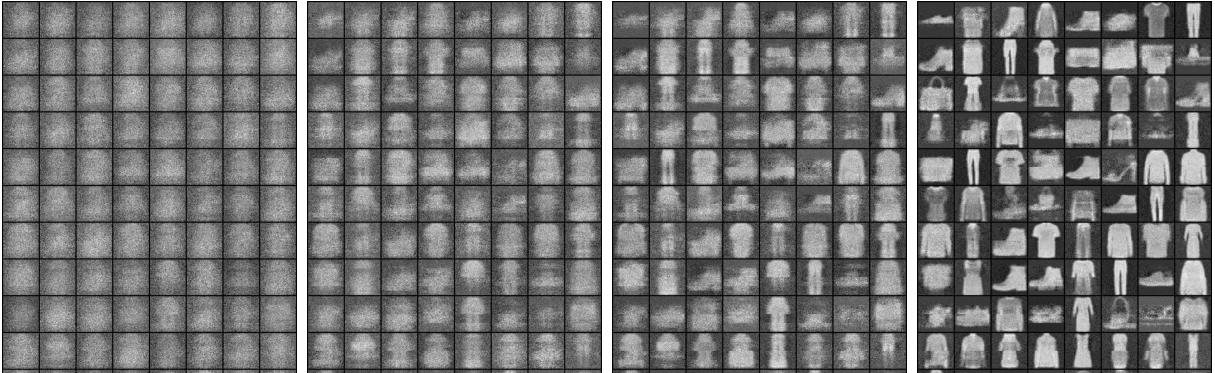
\includegraphics[width=0.55\columnwidth]{figures/fmnist2.pdf}
\label{fig:fashionmnist}	
}\hfill
\subfigure[]{
\includegraphics[width=0.41\columnwidth]{figures/mnist.pdf}
\label{fig:fashionmnist}	
}
\caption{Applying SWF on the Fashion MNIST dataset.}
\end{figure}

% \begin{figure}
% \begin{centering}
%   \setlength\tabcolsep{1pt}

% \begin{tabular}{cccc|c}
% $k=200$ & $k=2000$ & $k=10000$ & $k=40000$ & target\tabularnewline
% \includegraphics[height=6cm]{figures/FashionMNIST/image_200} & \includegraphics[height=6cm]{figures/FashionMNIST/image_2000} & \includegraphics[height=6cm]{figures/FashionMNIST/image_10000} & \includegraphics[height=6cm]{figures/FashionMNIST/image_38400} & \includegraphics[height=6cm]{figures/FashionMNIST/dataset_example}\tabularnewline
% \end{tabular}
% \par\end{centering}
% \caption{Applying SWF on the Fashion MNIST dataset.\label{fig:fashionmnist}}
% \end{figure}

On figure \ref{fig:fashionmnist}, we can see that a few thousand iterations of SWF is sufficient to get generated samples that capture most features of the training data. We note however that we are currently missing generation of fine-grained textures. We also display the SW2 loss of this run along iterations. Interestingly, such an experiment requires around $1h$ of computing power for a laptop computer on CPU, to be compared with the important ressources required by many other generative models.

% \end{itemize}



% \begin{figure}
% \begin{subfigure}[t]{0.5\textwidth}
% \begin{centering}
% \setlength\tabcolsep{1pt}
% \begin{tabular}{ccc|c}
% $k=1$ & $k=7$ & $k=70$ & target\tabularnewline
% \includegraphics[width=2cm]{figures/toy_save/output_dist_k=1-crop.pdf} & \includegraphics[width=2cm]{figures/toy_save/output_dist_k=20-crop.pdf} & \includegraphics[width=2cm]{figures/toy_save/output_dist_k=70-crop.pdf} &  \includegraphics[width=2cm]{figures/scatter_output_particles_k=70-crop.pdf}\tabularnewline
% \includegraphics[width=2cm]{figures/toy_load/output_dist_k=1-crop.pdf} & \includegraphics[width=2cm]{figures/toy_load/output_dist_k=20-crop.pdf} & \includegraphics[width=2cm]{figures/toy_load/output_dist_k=70-crop.pdf} &  \includegraphics[width=2cm]{figures/target-crop.pdf}\tabularnewline
% \end{tabular}
% % \par
% \end{centering}
% \caption{Toy example.}
% \label{fig:toy_example}
% \end{subfigure}
% \end{figure}

% \begin{figure}
% \begin{centering}
% \setlength\tabcolsep{1pt}
% \begin{tabular}{cccccc}
% $\lambda=0$ & $\lambda=0.1$ & $\lambda=0.2$ & $\lambda=0.3$ & $\lambda=0.5$ & $\lambda=1$\tabularnewline
% \includegraphics[width=2cm]{figures/supplementary/regularization/r0_output_dist_k=70-crop.pdf} & \includegraphics[width=2cm]{figures/supplementary/regularization/r01_output_dist_k=70-crop.pdf} & \includegraphics[width=2cm]{figures/supplementary/regularization/r02_output_dist_k=70-crop.pdf} &  \includegraphics[width=2cm]{figures/supplementary/regularization/r03_output_dist_k=70-crop.pdf}&  \includegraphics[width=2cm]{figures/supplementary/regularization/r05_output_dist_k=70-crop.pdf} &  \includegraphics[width=2cm]{figures/supplementary/regularization/r1_output_dist_k=70-crop.pdf}
% \end{tabular}
% \par
% \end{centering}
% \caption{Influence of the regularization parameter $\lambda$. The higher $\lambda$, the more entropic the output distribution.\label{fig:lambda_supp}}
% \end{figure}








% \newcommand{\ww}{0.2}


% \begin{minipage}{\linewidth}
% \begin{minipage}{0.4\textwidth}
% \begin{figure}[H]
% \centering
% \begin{tabular}{ccc|c}
% $k=1$ & $k=7$ & $k=70$ & target\tabularnewline
% \includegraphics[width=0.1\columnwidth]{figures/toy_save/output_dist_k=1-crop.pdf} & \includegraphics[width=0.1\columnwidth]{figures/toy_save/output_dist_k=20-crop.pdf} & \includegraphics[width=0.1\columnwidth]{figures/toy_save/output_dist_k=70-crop.pdf} &  \includegraphics[width=0.1\columnwidth]{figures/scatter_output_particles_k=70-crop.pdf}\tabularnewline
% \includegraphics[width=0.1\columnwidth]{figures/toy_load/output_dist_k=1-crop.pdf} & \includegraphics[width=0.1\columnwidth]{figures/toy_load/output_dist_k=20-crop.pdf} & \includegraphics[width=0.1\columnwidth]{figures/toy_load/output_dist_k=70-crop.pdf} &  \includegraphics[width=0.1\columnwidth]{figures/target-crop.pdf}\tabularnewline
% \end{tabular}
% \par
% \caption{Toy example: training data $y_i$ consists in $50 000$ samples drawn from a Gaussian Mixture Model with $20$ components of random weights, covariances and locations. \textbf{Left:} Output distribution for learning (top) and testing (bottom) particles. \textbf{Right:} (top) Close-up of some generated samples in red superimposed with learning points in black. (bottom) Target distribution. $N_\theta=30$, $N=3000$, $h=1$, $\lambda=10^{-4}$.
% \label{fig:toy_example}}
% \end{figure}
% \end{minipage}
% %
% \begin{minipage}{0.49\textwidth}
% \begin{figure}[H]
% \centering
% \begin{tabular}{cccc|c}
% $k=2K$ & $k=20K$ & $k=10K$ & $k=40K$ & target\tabularnewline
% \includegraphics[width=\ww\columnwidth]{figures/FashionMNIST/image_200} & \includegraphics[width=\ww\columnwidth]{figures/FashionMNIST/image_2000} & \includegraphics[width=\ww\columnwidth]{figures/FashionMNIST/image_10000} & \includegraphics[width=\ww\columnwidth]{figures/FashionMNIST/image_38400} & \includegraphics[width=\ww\columnwidth]{figures/FashionMNIST/dataset_example}\tabularnewline
% \end{tabular}
% \par
% \caption{Applying SWF on the Fashion MNIST dataset.
% \label{fig:fashionmnist}}
% \end{figure}
% \end{minipage}
% \end{minipage}


%!TEX root = ./icml_2019_sketchmcmc.tex

\section{Conclusion and Future Directions}

In this study, we proposed SWF, an efficient, nonparametric IGM algorithm.
SWF is based on formulating IGM as a functional optimization problem in Wasserstein spaces, where the aim is to find a probability measure that is close to the data distribution as much as possible while maintaining the expressiveness at a certain level.
SWF lies in the intersection of OT, gradient flows, and SDEs, which allowed us to convert the IGM problem to an SDE simulation problem. We provided finite-time bounds for the infinite-particle regime and established explicit links between the algorithm parameters and the overall error.
%We believe that the proposed algorithm is the first nonparametric IGM algorithm with explicit theoretical guarantees.
%
We conducted several experiments, where we showed that the results support our theory: SWF is able to generate samples from non-trivial distributions with low computational requirements.

The SWF algorithm opens up interesting future directions: (i) extension to differentially private settings \cite{dwork2014algorithmic} by exploiting the fact that it only requires random projections of the data, (ii) showing the convergence scheme of the particle system \eqref{eqn:sde_particle} to the original SDE \eqref{eqn:sde}, (iii) providing bounds directly for the particle scheme \eqref{eqn:euler_particle}.
% (iv) combining SWF with existing IGM approaches in order to be able to simulate the particles in lower dimensional space.






\bibliography{./references.bib}
\bibliographystyle{unsrt}

\addcontentsline{toc}{section}{Appendix}
\section*{Appendix}

%!TEX root = ./nips_2018_sketchmcmc_supp.tex

\section{Construction of the entropy-regularized gradient-flow}

We let $\mathcal{F}_{\lambda}(\mu) = \frac{1}{2} SW_2^2(\mu, \nu) + \lambda H(\mu)$ for a chosen reference measure $\nu$.

\begin{lemma}
Let $\nu$ be a probability measure on $\cB(0,1)$ with a strictly positive smooth density. Fix a time step $h > 0$, regularization constant $\lambda > 0$ and a radius $r > \sqrt{d}$. For a probability measure $\mu_0$ on $B(0, r)$ with density $\rho_0 \in L^{\infty}$, there is a probability measure $\mu$ on $\overline{B}(0,r)$ minimizing:
\[
\mathcal{G}(\mu) = \mathcal{F}_{\lambda} (\mu) + \frac{1}{2h} W_2^2(\mu, \mu_0) 
\]
Moreover the optimal $\mu$ has a density $\rho$ on $B(0,r)$ and:
\begin{equation} \label{ineq:inf_norm_bound}
||\rho||_{L^{\infty}} \leq (1 + h/\sqrt{d})^d ||\rho_0||_{L^{\infty}}
\end{equation}
\end{lemma}
\begin{proof}
The set of measures supported on $\cB(0,r)$ is compact in the topology given by $W_2$ metric. Furthermore it is well known [[some ref]] that functional $H$ is lower semicontinuous in this topology. Since $SW_2$ is a distance function [[Bonnotte]], dominated by $\frac{1}{\sqrt{d}} W_2$ [[Bonnotte]] we have:
\[
|SW_2(\pi_0, \nu) - SW_2(\pi_1, \nu)| \leq SW_2(\pi_0, \pi_1) \leq \frac{1}{\sqrt{d}}W_2(\pi_0, \pi_1).
\]
The above means that $SW_2(\cdot, \nu)$ is continuous with respect to topology given by $W_2$, which implies that $SW_2^2(\cdot, \nu)$ is continuous in this topology as well. Therefore $G$ is a lower semicontinuous function on a compact set, bounded from below. Hence there exists a minimum  $\mu$ of $G$ on $\mathcal{P}(\cB(0,r))$. Furthermore, since $H(\pi) = +\infty$  for measures $\pi$ that do not admit a density with respect to Lebesgue measure, the measure $\mu$ must admit a density $\rho$.

If $\rho_0$ is smooth and positive on $B(0,r)$, the inequality \ref{ineq:inf_norm_bound} is true by [[Bonnotte]] Lemma 5.4.3. When $\rho_0$ is just in $L^{\infty}(\cB(0,r))$, we proceed by smoothing. Let $\mu_t$ be the heat flow on $\cB(0,r)$ starting from $\mu_0$ ([[some ref on existance?]]). Then for any $t > 0$, $\mu_t$ has a smooth density $\rho_t$ such that $||\rho_t||_{L^{\infty}} \leq ||\rho_0||_{L^{\infty}}$. Let $\hat{\mu_t}$ be the minimum of $ \mathcal{F}_{\lambda}(\cdot) + \frac{1}{2h} W_2^2(\cdot, \mu_t)$, and let $\hat{\rho_t}$ be the density of $\hat{\mu_t}$. Using [[Bonnotte]] Lemma 5.4.3 we get 
\[
||\hat{\rho_t} ||_{L^{\infty}} \leq (1 + h\sqrt{d})^d ||\rho_t||_{L^{\infty}} \leq (1 + h\sqrt{d})^d ||\rho_0||_{L^{\infty}}
\]
and so for all $t>0$ densities $\hat{\rho_t}$ lie in a ball of finite radius in $L^{\infty}$.  Using compactness of $\mathcal{P}(\cB(0,r))$ in weak topology and compactness of closed ball in $L^{\infty}(\cB(0,r))$ in weak star topology, we can choose a sequence $(t_k)_{k \geq 1}$  of positive numbers such that $\lim_{k \rightarrow \infty} t_k = 0$ and $\hat{\mu}_{t_k} , \hat{\rho}_{t_k}$ converge along that subsequence to limits $\hat{\mu}$, $\hat{\rho}$. Obviously $\hat{\rho}$ is the density of $\hat{\mu}$, since for any continuous function $f$  on $\cB(0,r)$ we have:
\[
\int \hat{\rho} f dx = \lim_{k \rightarrow \infty} \int \rho_{t_k} f dx = \lim_{k \rightarrow \infty} \int f d\mu_{t_k} = \int f d\mu
\]
Furthermore, since $\hat{\rho}$ is the weak star limit of a bounded subsequence, it obeys the same bound as subsequence, that is:
\[
||\hat{\rho} ||_{L^{\infty}} \leq (1 + h\sqrt{d})^d ||\rho_0||_{L^{\infty}}
\]
To finish, we just need to prove that $\hat{\mu}$ is a minimum of $G$. We remind our reader, that we already established existence of some minimum $\mu$ (that might be different from $\hat{\mu}$). Since $\hat{\mu}_{t_k}$ converges weakly to $\hat{\mu}$ in $\mathcal{P}(\cB(0,r))$, it implies convergence of second moments (because $x^2$ is continuous and bounded on $\cB(0,r)$), and hence convergence in $W_2$ as well. Similarly $\mu_{t_k}$ converges to $\mu_0$ in $W_2$. Using the lower semicontinuity of $G$ we now have:
\[
\begin{aligned}
\mathcal{F}_{\lambda}(\hat{\mu}) + \frac{1}{2h} W_2^2(\hat{\mu}, \mu_0)  & \leq \liminf_{k \rightarrow \infty} \left( \mathcal{F}_{\lambda}(\hat{\mu}_{t_k}) + \frac{1}{2h} W_2^2(\hat{\mu}_{t_k} , \mu_0) \right) \\
& \leq \liminf_{k \rightarrow \infty}  \mathcal{F}_{\lambda}(\mu) + \frac{1}{2h} W_2^2(\mu , \mu_{t_k})   \\
& + \frac{1}{2h}  W_2^2(\hat{\mu}_{t_k}, \mu_0) - \frac{1}{2h} W_2^2(\hat{\mu}_{t_k}, \mu_{t_k})   \\
& = \mathcal{F}_{\lambda} (\mu) + \frac{1}{2h} W_2^2(\mu, \mu_0) 
\end{aligned}
\]
where the second inequality comes from the fact, that $\hat{\mu}_{t_k}$ minimizes $\mathcal{F}_{\lambda}(\cdot) + \frac{1}{2h}W_2^2(\cdot, \mu_{t_k})$. From the above inequality and previously established facts, it follows that $\hat{\mu}$ is a minimum of $G$ with density satisfying \ref{ineq:inf_norm_bound}.
\end{proof}

Existance of gradient flow (generalized minimizing movement scheme)
\begin{thm} \label{thm:existance_gmm_scheme}
Let $\nu$ be a probability measure on $\cB(0,1)$ with a strictly positive smooth density. Choose a regularization constant $\lambda > 0$ and radius $r > \sqrt{d}$. Given an absolutely continuous measure $\mu_0 \in \mathcal{P}(\cB(0,r))$ with density $\rho_0 \in L^p$, there is a Lipschitz generalized minimizing movement scheme $(\mu_t)_{t\geq 0}$ in $\mathcal{P}(\cB(0,r))$ starting from $\mu_0$ for the functional:
\[
\mathcal{F}(h, n , \mu_+, \mu_-) = \mathcal{F}_{\lambda}(\mu_+) + \frac{1}{2h}W_2^2(\mu_+, \mu_-)
\]
Morover for time $t > 0$ measure $\mu_t$ has density $\rho_t$ and:
\[
||\rho_t||_{L^p} \leq e^{t\sqrt{d}}/q ||\rho_0||_{L^p}
\]
\end{thm}
\begin{proof}
The proof is exactly the same as the proof of Theorem 5.5.3 in [[Bonnotte]], but we include it for completeness   ........
\end{proof}

\begin{thm}
Let $\mu_t$ be a generalized minimizing movement scheme given by \ref{thm:existance_gmm_scheme}. We denote by $\rho_t$ the denisty of $\mu_t$. Then $\rho_t$ satisfies the continuity equation:
\[
\frac{\partial \rho_t}{\partial t} + \text{div}(v_t \rho_t) = \lambda \Delta \rho_t  \quad \quad \quad v_t(x) = - \int_{S^{d-1}} \psi_{t, \theta}'(\langle x , \theta \rangle ) \theta d\theta 
\]
in a weak sense.
\end{thm}
%!TEX root = ./nips_2018_sketchmcmc_supp.tex

\section{The Gradient Flow and the SDE}

Let $\rho_t$ be the density of a measure $\mu_t$ with respect to the Lebesgue measure, such that $\mu_t(dx) = \rho_t(x) dx$. In this section, we will be interested in the following gradient flow in $\W$:
\begin{align}
\partial_t \rho_t &= - \nabla_{\W} \F_\lambda(\rho_t) \\
&=  \nabla \cdot (\rho_t \> v_t) + \lambda \Delta \rho_t, \label{eqn:gradflow_reg}
\end{align}
where 
\begin{align}
v_t(x) \triangleq \nabla \Psi_t(x) = \int_{\Sp^{d-1}} \psi'_{t,\theta}(\langle \theta, x \rangle) \theta \> d\theta \label{eqn:idt_v}
\end{align}
and
\begin{align}
\Psi_t(x) \triangleq \int_{\mathbb{S}^{d-1}} \psi_{t,\theta}(\langle \theta, x \rangle) \> d\theta.
\end{align}
Here, $\psi_{t,\theta}$ denotes the Kantorovich potential between $\theta^*_{\#}\mu_t$ and $\theta^*_{\#}\nu$ and $d\theta$ represents the uniform probability measure on $\Sp^{d-1}$, such that $\int_{\Sp^{d-1}} d \theta = 1$.

We now consider the modified flow given in \eqref{eqn:gradflow_reg}. We can observe that, this equation is the Fokker-Planck equation associated with the following stochastic differential equation (SDE):
\begin{align}
d X_t = - v_t(X_t) dt + \sqrt{2 \lambda } d W_t, \label{eqn:sde}
\end{align}
where $W_t$ denotes the standard Brownian motion.

\begin{assumption}
\label{asmp:sde_ergo}
For all $\lambda >0$, the SDE  \eqref{eqn:sde} has a unique strong solution denoted by $(X_t)_{t\geq 0}$ for any starting point $x \in \R^d$. Its define a non-homogenous Markov semi-group $(P_{s,t})_{t\geq s\geq 0}$ which admits a unique invariant measure denoted by $\nu_\lambda$. % and it is geometrically ergodic. 
\end{assumption}

\begin{assumption}
\label{asmp:sde_expconv}
The probability measure of the diffusion $(\mu_t)_{t\geq 0}$ converges exponentially fast to its invariant measure $\nu_\lambda$, such that there exists $C_0, C_1 >0$
\begin{align}
\|\mu_t - \nu_\lambda \|_{\TV} \leq C_0 \exp(-C_1 t \lambda).
\end{align}
\end{assumption}

We first provide a bound between the invariant measure $\nu_\lambda$ and $\nu$.

\begin{prop}
\label{prop:dist_statmeas}
Consider the following SDE
\begin{align}
d Y_t = - v_t(Y_t) dt + \sqrt{2 \epsilon } d W_t. \label{eqn:sde_eps}
\end{align}
Assume that it satisfies \Cref{asmp:sde_ergo} with the invariant measure denoted by $\nu_\epsilon$. Let $\rho^\epsilon_t$ denote the probability density function of $Y_t$ at time $t$. Further assume that for all $\epsilon,t>0$, there exists $C >0$  
\begin{align}
\int_{0}^t \int_{\R^d} \frac{\|\nabla \rho^\epsilon_s(x) \|^2}{\rho^\epsilon_s(x)} dx ds <C, \qquad \text{and} \qquad \int_{0}^t \int_{\R^d}  \frac{\|\nabla \rho^\epsilon_s(x)\|}{1+\|x\|} dx ds <\infty.
\end{align}
Then the following bound holds:
\begin{align}
\lim_{\epsilon \rightarrow 0} \| \nu_\lambda - \nu_\epsilon \|_{\TV}^2 \leq 2 C \lambda.
\end{align}
\end{prop}
%
\begin{proof}
By Corollary 1.2 of \cite{bogachev2016distances}, for any $\epsilon > 0$ we have 
\begin{align}
\| \nu_\lambda - \nu_\epsilon \|_{\TV}^2 &\leq \int_0^\infty \int_{\R^d} \Bigl| \Bigl(\frac{\sqrt{\lambda}}{\sqrt{\epsilon}}- \frac{\sqrt{\epsilon}}{\sqrt{\lambda}} \Bigr) \sqrt{2\epsilon}  \Bigr|^2 \frac{\|\nabla \rho^\epsilon_s(x)\|^2}{\rho^\epsilon_s(x)}  dx ds \\
&\leq  C \Bigl| \Bigl(\frac{\sqrt{\lambda}}{\sqrt{\epsilon}}- \frac{\sqrt{\epsilon}}{\sqrt{\lambda}} \Bigr) \sqrt{2\epsilon}  \Bigr|^2 \label{eqn:prop_interm} \\
&= \frac{2C}{\lambda} (\lambda - \epsilon)^2,
\end{align}
where \eqref{eqn:prop_interm} is obtained by the assumption. The desired result is obtained by taking the taking the limit of both sides. 
\end{proof}
%



\section{Euler Discretization}


Corollary~\ref{prop:dist_statmeas} shows that if we could simulate \eqref{eqn:sde}, then we could use the sample paths $(X_t)_t$ as
samples drawn from $\nu_\lambda$, which is not far from $\nu$. However, this is not possible since the drift $v_t$ cannot be computed analytically, and the SDE \eqref{eqn:sde} is a continuous-time process.

We now consider the approximate Euler-Maruyama discretization, that is given as follows:
\begin{align}
\bar{X}_{k+1} = \bar{X}_k - h \hat{v}_k(\bar{X}_k) + \sqrt{2 \lambda h} Z_{k+1},
\end{align}
where $k \in \mathbb{N}_+$ denotes the iteration number, $\{Z_k\}_{k}$ denotes a series of standard Gaussian random variables, $h$ denotes the step-size, and $\hat{v}_k$ is a computable unbiased estimator of $v_{kh}$.


By Theorem 5.6.1 of \cite{bonnotte2013unidimensional}, we know that $\Psi_t$ is Lipschitz continuous. We consider the following assumptions:
\begin{assumption}
\label{asmp:lipschitz}
The drift is Lipschitz continuous, i.e.\ there exits $L < \infty$ such that
\begin{align}
\| v_t(x) - v_{t'}(x') \| \leq L ( \|x-x' \| + |t-t'|).
\end{align}
\end{assumption}
%
\begin{assumption}
\label{asmp:dissip}
For all $t \geq 0$, $v_t$ is dissipative, i.e. for all $x \in \R^d$.
\begin{align}
\langle x, v_t(x) \rangle \geq m \|x\|^2 -b
\end{align}
for some $m,b >0$.
\end{assumption}
%
\begin{assumption}
\label{asmp:stochgrad}
The estimator of the drift is unbiased, i.e.\ $\E[\hat{v}_t] = v_t$ for all $t \geq 0$, and its variance satisfies the following condition for some $\delta \in (0,1)$ and for all $t\geq 0$, $x \in \R^d$:
\begin{align}
\E[ \|\hat{v}_t(x) - v_t(x) \|^2] \leq 2 \delta(L^2 \|x\|^2 + B^2).
\end{align}
\end{assumption}
%
\begin{assumption}
\label{asmp:init_fun}
The function $\Psi_t$ satisfies the following conditions for all $t \geq 0$:
\begin{align}
|\Psi_t(0)| \leq A, \qquad \text{and} \qquad \|v_t(0)\| \leq B
\end{align}
for $A,B \geq 0$.
\end{assumption}


We are interested in computing the distance $\| \muh_{Kh} - \nu_\lambda \|_{\TV}$, where $\muh_{Kh}$ denotes the law of $\bar{X}_K$ with step size $h$. In order to upper-bound this distance, we follow the approach presented in \cite{dalalyan2017theoretical} and \cite{raginsky17a}, where we decompose the into two terms: $\| \muh_{Kh} - \nu_\lambda \|_{\TV} \leq \| \muh_{Kh} - \mu_t \|_{\TV} + \| \mu_{T} - \nu_\lambda \|_{\TV}$, where $\mu_T$ denotes the law of $X_T$ such that $T=Kh$. %$(X_t)_t$ is the solution of the continuous-time SDE \eqref{eqn:sde} and 

We start by upper-bounding the first term. 
%
\begin{lemma}
\label{lem:euler}
Assume that the conditions \Cref{asmp:lipschitz,asmp:stochgrad,asmp:dissip,asmp:init_fun} hold. Then, the following bound holds:
\begin{align}
\| \muh_{Kh} - \mu_{T} \|_{\TV}^2 \leq \frac{L^2 K}{4\lambda} \Bigl( \frac{C_1 h^3}{3} + 3 \lambda d h^2 \Bigr) + \frac{C_2 \delta K h}{8\lambda},
\end{align}
where the constants $C_1$ and $C_2$ are explicitly defined in the proof. 
\end{lemma}
%
%
\begin{proof}
We use the proof technique presented in \cite{dalalyan2017theoretical,raginsky17a}. Starting from the discrete-time process $(\bar{X}_k)_{k\in \mathbb{N}_+}$, we first define a continuous-time process $(Y_t)_{t\geq 0}$ that linearly interpolates $(\bar{X}_k)_{k\in \mathbb{N}_+}$, given as follows: 
\begin{align}
d Y_t = \tilde{v}_t(Y) dt + \sqrt{2 \lambda} dW_t, \label{eqn:sde_linear}
\end{align}
where $\tilde{v}_t(Y) \triangleq - \sum_{k=0}^{\infty} \hat{v}_k (Y_{kh}) \mathds{1}_{[kh, (k+1)h)}(t)$ and $\mathds{1}$ denotes the indicator function. It is easy to verify that for all $k \in \mathbb{N}_+$, we have $Y_{kh} = \bar{X}_k$. 

Let us denote the distributions of $(X_t)_{t \in [0,T]}$ and $(Y_t)_{t \in [0,T]}$ as $\pi_{X}^T$ and $\pi_{Y}^T$ with $T = Kh$. Then we can use Girsanov's formula to express the Kullback-Leibler (KL) divergence between these two distributions, given as follows:
\begin{align}
\KL (\pi_{X}^T || \pi_{Y}^T) &= \frac1{4 \lambda} \int_0^{Kh} \E[ \|v_t(Y_t) + \tilde{v}_t(Y) \|^2 ]  \> dt \\
&= \frac1{4 \lambda} \sum_{k=0}^{K-1} \int_{kh}^{(k+1)h} \E[ \|v_t(Y_t) + \tilde{v}_t(Y) \|^2 ] \> dt \\
&= \frac1{4 \lambda} \sum_{k=0}^{K-1} \int_{kh}^{(k+1)h} \E[ \|v_t(Y_t) - \hat{v}_{kh}(Y_{kh}) \|^2 ] \> dt,
\end{align}
where we use the notation $\hat{v}_{kh} \equiv \hat{v}_{k}$ in order to illustrate the time index more explicitly. By using $v_t(Y_t) - \hat{v}_{kh}(Y_{kh}) = ( v_t(Y_t) - v_{kh}(Y_{kh})) + ( v_{kh}(Y_{kh}) - \hat{v}_{kh}(Y_{kh}))$, we obtain
%
\begin{align}
\nonumber \KL (\pi_{X}^T || \pi_{Y}^T) \leq& \frac1{2 \lambda} \sum_{k=0}^{K-1} \int_{kh}^{(k+1)h} \E[ \|v_t(Y_t) - {v}_{kh}(Y_{kh}) \|^2 ] \> dt \\
&+  \frac1{2 \lambda} \sum_{k=0}^{K-1} \int_{kh}^{(k+1)h} \E[ \|v_{kh}(Y_{kh}) - \hat{v}_{kh}(Y_{kh}) \|^2 ] \> dt \\
\nonumber \leq& \frac{L^2}{\lambda} \sum_{k=0}^{K-1} \int_{kh}^{(k+1)h} \bigl(\E[ \|Y_t - Y_{kh} \|^2 ] + (t-kh)^2 \bigr)  \> dt \\
&+  \frac1{2 \lambda} \sum_{k=0}^{K-1} \int_{kh}^{(k+1)h} \E[ \|v_{kh}(Y_{kh}) - \hat{v}_{kh}(Y_{kh}) \|^2 ] \> dt . \label{eqn:lem1_proof_interm}
\end{align}
The last inequality is due to the Lipschitz condition \Cref{asmp:lipschitz}.

Now, let us focus on the term $\E[ \|Y_t - Y_{kh} \|^2]$. By using \eqref{eqn:sde_linear}, we obtain:
\begin{align}
Y_t - Y_{kh} = - (t-kh) \hat{v}_{kh}(Y_{kh}) + \sqrt{2 \lambda (t-kh)} Z,
\end{align}
where $Z$ denotes a standard normal random variable. By adding and subtracting the term $-(t-kh) v_{kh}(Y_{kh})$, we have:
\begin{align}
Y_t - Y_{kh} = -(t-kh)v_{kh}(Y_{kh}) + (t-kh)(v_{kh}(Y_{kh}) - \hat{v}_{kh}(Y_{kh})) + \sqrt{2 \lambda (t-kh)} Z.
\end{align}
Taking the square and then the expectation of both sides yields:
\begin{align}
\nonumber \E[ \|Y_t - Y_{kh} \|^2] \leq& 3(t-kh)^2 \E[ \|v_{kh}(Y_{kh})\|^2] + 3 (t-kh)^2 \E[\|v_{kh}(Y_{kh}) - \hat{v}_{kh}(Y_{kh})\|^2] \\
&+ 6\lambda (t-kh)d.
\end{align}
As a consequence of \Cref{asmp:lipschitz} and \Cref{asmp:init_fun}, we have $\| v_t(x)\| \leq L\|x\|+B$ for all $t \geq 0$, $x\in \R^d$. Combining this inequality with \Cref{asmp:stochgrad}, we obtain:
\begin{align}
\nonumber \E[ \|Y_t - Y_{kh} \|^2] \leq& 6(t-kh)^2 (L^2 \E[ \|Y_{kh}\|^2] + B^2) + 6(t-kh)^2 (L^2 \E[ \|Y_{kh}\|^2] + B^2) \\
&+ 6\lambda (t-kh)d\\
=& 12(t-kh)^2 (L^2 \E[ \|Y_{kh}\|^2] + B^2) + 6\lambda (t-kh)d.
\end{align}
By Lemma 3.2 of \cite{raginsky17a}, we have $\E[ \|Y_{kh}\|^2] \leq C_0 \triangleq C_e +2  (1 \vee \frac1{m})(b+2B^2 + d \lambda)$, where $C_e$ denotes the entropy of $\mu_0$. Using this result in the above equation yields:
\begin{align}
\E[ \|Y_t - Y_{kh} \|^2] \leq& 12(t-kh)^2 (L^2 C_0 + B^2) + 6\lambda (t-kh)d. \label{eqn:lem_bound1}
\end{align}

We now focus on the term $\E[ \|v_{kh}(Y_{kh}) - \hat{v}_{kh}(Y_{kh}) \|^2 ]$ in \eqref{eqn:lem1_proof_interm}. Similarly to the previous term, we can upper-bound this term as follows:
\begin{align}
\E[ \|v_{kh}(Y_{kh}) - \hat{v}_{kh}(Y_{kh}) \|^2 ] \leq& 2 \delta(L^2 \E[\|Y_{kh}\|^2] + B^2) \\
\leq& 2 \delta(L^2 C_0 + B^2). \label{eqn:lem_bound2}
\end{align}

By using \eqref{eqn:lem_bound1} and \eqref{eqn:lem_bound2} in \eqref{eqn:lem1_proof_interm}, we obtain:
\begin{align}
\nonumber \KL (\pi_{X}^T || \pi_{Y}^T) \leq& \frac{L^2}{\lambda} \sum_{k=0}^{K-1} \int_{kh}^{(k+1)h} \bigl(12(t-kh)^2 (L^2 C_0 + B^2) + 6\lambda (t-kh)d +(t-kh)^2 \bigr) dt\\
&+  \frac1{2 \lambda} \sum_{k=0}^{K-1} \int_{kh}^{(k+1)h} 2 \delta(L^2 C_0 + B^2) \> dt \\
=& \frac{L^2 K}{\lambda} \Bigl( \frac{C_1 h^3}{3} + \frac{6 \lambda d h^2}{2} \Bigr) + \frac{C_2 \delta K h}{2\lambda},
\end{align}
where $C_1 = 12(L^2 C_0 + B^2)+1$ and $C_2 = 2 (L^2 C_0 + B^2)$.

Finally, by using the data processing and Pinsker inequalities, we obtain:
\begin{align}
\| \muh_{Kh} - \mu_{T} \|_{\TV}^2 \leq \| \pi_{X}^T - \pi_{Y}^T \|_{\TV}^2 \leq& \frac1{4} \KL (\pi_{X}^T || \pi_{Y}^T) \\
=& \frac{L^2 K}{4\lambda} \Bigl( \frac{C_1 h^3}{3} + 3 \lambda d h^2 \Bigr) + \frac{C_2 \delta K h}{8\lambda}.
\end{align}
This concludes the proof.

\end{proof}


\begin{thm}
Assume that \Cref{asmp:sde_ergo,asmp:sde_expconv,asmp:lipschitz,asmp:stochgrad,asmp:dissip,asmp:init_fun} hold. Then, the following bound holds:
\begin{align}
\| \muh_{K} - \nu_\lambda \|_{\TV} \leq \left \lbrace  \frac{L^2 K}{4\lambda} \Bigl( \frac{C_1 h^3}{3} + 3 \lambda d h^2 \Bigr) + \frac{C_2  \delta K h}{8\lambda} \right \rbrace^{1/2} +  C_3 \exp(-C_4 Kh \lambda),
\end{align}
for some $C_1,C_2,C_3,C_4 > 0$.
\end{thm}
%
\begin{proof}
The proof is a direct consequence of the triangle inequality, Lemma~\ref{lem:euler}, and assumption \Cref{asmp:sde_expconv}.
\end{proof}

\begin{cor}
  \label{coro:precision}
  Assume that \Cref{asmp:sde_ergo,asmp:sde_expconv,asmp:lipschitz,asmp:stochgrad,asmp:dissip,asmp:init_fun} hold. Then for all $\varepsilon >0$, setting
  \begin{align}
T = Kh  = \ceil{-\log(\varepsilon/(2C_3))/(C_4\lambda)} \, , \qquad 
h = (3/C_1)\wedge\left(\frac{\varepsilon^2 \lambda}{L^2 T}(1+3\lambda d)^{-1}\right) \,,
  \end{align}
  we have
  \begin{align}
    \| \muh_{K} - \nu_\lambda \|_{\TV} \leq \varepsilon + \left(\frac{C_2 \delta K h}{8\lambda}\right)^{1/2} . 
  \end{align}
\end{cor}
\begin{proof}
Considering the bound given in Lemma~\ref{lem:euler}, the choices of $T$ and $h$ imply that
\begin{align}
\frac{L^2 K}{4\lambda} \Bigl( \frac{C_1 h^3}{3} + \frac{6 \lambda d h^2}{2} \Bigr) \leq \frac{\varepsilon^2}{4}, \quad \text{and} \quad C_3 \exp(-C_4 Kh \lambda) \leq \frac{\varepsilon}{2}.
\end{align}
?

\end{proof}

\section{Discussion on the assumptions}

\umut{This section will be rewritten.}

\subsection{Conditions for the unique solution to the flow}

The following conditions ensure that there is a unique solution to the flow given in \eqref{eqn:gradflow_reg}:
\begin{assumption}
\label{asmp:flowunq_1}
There exists $p>d+2$ such that for every open ball $B \subset \R^d$, one has
\begin{align}
\int_0^T \int_B \|v_t(x)\|^p dx\> dt < \infty.
\end{align}
\end{assumption}
%
\begin{assumption}
\label{asmp:flowunq_2}
The initial measure $\mu_0$ has finite entropy, such that
\begin{align}
\int_{\R^d} \rho_0(x) \log \rho_0(x) dx < \infty,
\end{align}
where $\mu_0(dx) = \rho_0(x)dx$ and $\rho_0 \in L^1(\R^d)$.
\end{assumption}
%
\begin{assumption}
\label{asmp:flowunq_3}
There exist $\alpha, \gamma, \delta, c, k \in \R_+$ such that for all $(t,x) \in [0,T] \times \R^d$ 
\begin{align}
\langle v_t(x), x \rangle \leq \gamma - (ck + \delta) \| x\|^{2k},
\end{align}
and 
\begin{align}
\label{asmp:flowunq_4}
\|v_t(x)\| \leq \alpha \exp(\frac{c}{2} \|x\|^{2k}), \qquad \text{and} \qquad \int_{\R^d} \exp(\frac{c}{2}\|x\|^{2k} ) \mu_0(dx) < \infty.
\end{align}
\end{assumption}

The following theorem ensures the uniqueness.
\begin{thm}[Theorem 3.3 \cite{bogachev2007uniqueness}]
Assume that \Cref{asmp:flowunq_1,asmp:flowunq_2,asmp:flowunq_3,asmp:flowunq_4} hold. Then, there exists a unique family $\{\mu_t, t\in(0,T]\}$ of probability measures on $\R^d$ solving \eqref{eqn:gradflow_reg}.
\end{thm}

\subsection{The assumptions of Proposition~\ref{prop:dist_statmeas}}

The assumptions of Proposition~\ref{prop:dist_statmeas} can be satisfied if we further assume certain regularity assumptions on $v_t$. For more information and a discussion about these assumptions, we refer the reader to Remark 1.4 in \cite{bogachev2016distances} and \cite{bogachev2006global,bogachev2008estimates}.



%%% Local Variables:
%%% mode: latex
%%% TeX-master: "nips_2018_sketchmcmc_supp"
%%% End:

%!TEX root = ./aistats_2019_sketchmcmc_supp.tex


% \section{Visual Comparison with Existing Approaches}

% In this section, we provide the results presented in \cite{deshpande2018generative} for visual comparison. These results are obtained by running different IGM approaches on the MNIST dataset, namely GAN \cite{goodfellow2014generative}, Wasserstein GAN (W-GAN) \cite{arjovsky2017wasserstein} and the Sliced-Wasserstein Generator (SWG) \cite{deshpande2018generative}.

% \begin{figure}[h!]
% \centering
% \includegraphics[width=0.5\columnwidth]{mnist_all.pdf}
% \caption{Performance of GAN (left), W-GAN (middle), SWG (right) on MNIST. (The figure is directly taken from \cite{deshpande2018generative}.) }
% \label{fig:mnistall}
% \end{figure}


\section{Additional Experimental Results}

\subsection{The Sliced Wasserstein Flow}
The whole code for the Sliced Wasserstein Flow was implemented in Python, for use with Pytorch\footnote{\url{www.pytorch.org}.}. The code was written so as to run efficiently on GPU, and is available on the publicly available repository related to this paper\footnote{\url{github.com/removed_for_double_blind}.}.

In practice, the SWF involves relatively simple operations, the most important being:
\begin{itemize}
  \item For each random $\theta\in\{\theta_n\}_{n=1\dots N_\theta}$,  compute its inner product with all items from a dataset and obtain the empirical quantiles for these \emph{projections}.
  \item At each step $k$ of the SWF, for each projection $z=\left<\theta, \bar{X}^i_k\right>$, apply two piece-wise linear functions, corresponding to the scalar optimal transport $\psi_{k, \theta}'(z)$.
\end{itemize}
Even if such steps are conceptually simple, the quantile and required linear interpolation functions were not available on GPU for any framework we could figure out at the time of writing this paper. Hence, we implemented them ourselves for use with Pytorch, and the interested reader will find them in the Github repository dedicated to this paper.

Given these operations, putting a SWF implementation together is straightforward, and the online code is able to apply it on any dataset.

\subsection{The need for dimension reduction through autoencoders}

In this study, we used an autoencoder trained on the dataset as a dimension reduction technique, so that the SWF is applied to transport particles in a latent space of dimension $d\approx 50$, instead of the orginial $d>1000$ of image data.

The curious reader may wonder why SWF is not applied directly on this original space, and what performances should be expected there. We have done this experiment, and we found out that SWF has much trouble rapidly converging to satisfying samples. In figure~\ref{fig:suppnoae}, we show the progressive evolution of particles undergoing SWF when the target is directly taken as the uncompressed dataset.

\begin{figure}
\centering
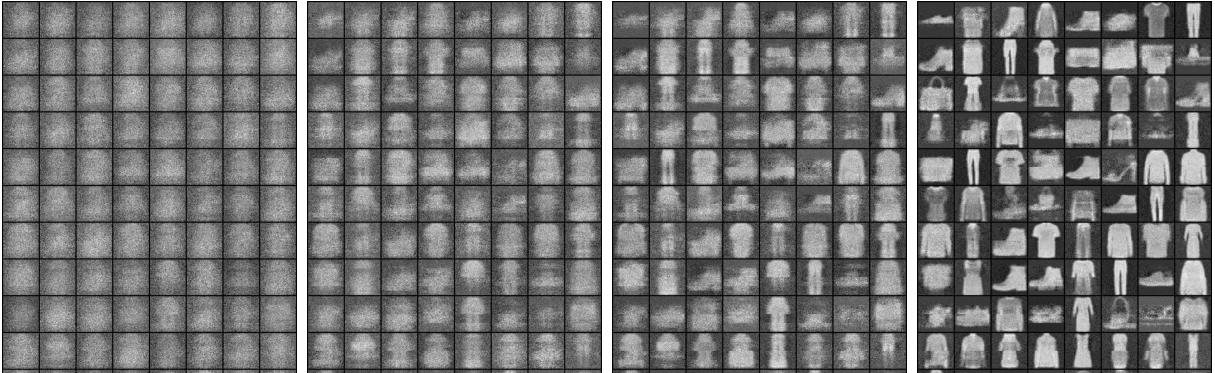
\includegraphics[width=\columnwidth]{figures/supplementary/fmnist_noae.pdf}
\includegraphics[width=\columnwidth]{figures/supplementary/mnist_noae.pdf}
\caption{The evolution of SWF through 15000 iterations, when the original high-dimensional data is kept instead of working on reduced bottleneck features as done in the main document. Showing results on the MNIST and FashionMNIST datasets.}
\label{fig:suppnoae}
\end{figure}

In this experiment, the strategy was to change the projections $\theta$ at each iterations, so that we ended up with a set of projections being $\{\theta_{n,k}\}_{n=1\dots N_\theta}^{k=1\dots K}$ instead of the fixed set of $N_\theta$ we now consider in the main document. This strategy is motivated by the complete failure we observed whenever we picked such fixed projections throughout iterations.

As may be seen on Figure~\ref{fig:suppnoae}, the particles definitely converge to samples from the desired datasets, and this is encouraging. However, we feel that the extreme number of iterations required to achieve such convergence comes from the fact that theory needs an integral over the $d-$dimensional sphere at each step of the SWF, which is clearly an issue whenever $d$ gets too large.
Although our solution of picking new samples from the sphere at each iteration alleviated this issue to some extent, the curse of dimensionality prevents us from doing much better with just thousands of projections at a time.

This being said, we are confident that good performance would be obtained if millions of projections could be considered for transporting such high dimensional data because i/ theory suggests it and ii/ we observed excellent performance on reduced dimensions.

However, we unfortunately did not have the computing power it takes for such large scale experiments and this is what motivated us in the first place to introduce some dimension-reduction technique through AE.

\subsection{Structure of our autoencoders for reducing data dimension}

As mentioned in the text, we used autoencoders to reduce the dimensionality of the transport problem. The structure of these networks is the following:

\begin{itemize}
  \item $\textbf{Encoder}$ Four 2d convolution layers with \(num_chan_out, kernel size, stride, padding\) being $(3,3,1,1)$, $(32,2,2,0)$, $(32,3,1,1)$, $(32, 3,1,1)$, each one followed by a relu activation. At the output, a linear layer gets the desired bottleneck size.

  \item $\textbf{Decoder}$ A linear layer gets from the bottleneck features to a vector of dimension $8192$, which is reshaped as $(32, 16,16)$. Then, three convolution layers are applied, all with $32$ output channels and \(kernel size, stride, panning\) being respectively $(3,1,1)$, $(3,1,1)$, $(2,2,0)$. A 2d convolution layer is then applied with an output number of channels being that of the data \($1$ for black and white, $3$ for colour\), and a \(kernel size, stride, panning\) as $(3,1,1)$. In any case, all layers are followed by a relu activation, and a sigmoid activation is applied a the very output.
\end{itemize}

Once these networks defined, these autoencoders are trained in a very simple manner by minimizing the squared differenc between input and output over the training set of the considered dataset (here MNIST or FashionMNIST). This training was achieved with the Adam algorithm \cite{kingma2014adam} with learning rate $1e-3$.

No additional training trick was involved as in Variational Autoencoder \cite{kingma2013VAE} to make sure the distribution of the bottleneck features match some prior. The core advantage of the proposed method in this respect is indeed to turn any previously learned AE as a generative model, by automatically and non-parameterically transporting particles drawn from an arbitrary prior distribution $\mu$ to the observed empirical distribution $\nu$ of the bottleneck features over the training set.

\subsection{Convergence plots of SWF}

\begin{figure}
\begin{centering}
\includegraphics[width=0.5\columnwidth]{figures/iterations.pdf}
\par\end{centering}
\caption{Approximately computed $\SW$ between the output $\bar{\mu}_{k}^{N}$ and data distribution $\nu$ in the MNIST experiment for different dimensions $d$ for the bottleneck features (and the corresponding pre-trained AE).
\label{fig:supptoy_sw}}
\end{figure}

In the same experimental setting as in the main document, we also illustrate the behavior of the algorithm for varying dimensionality $d$ for the bottleneck-features. To monitor the convergence of SWF as predicted by theory, we display the approximately computed $\SW$ distance between the distribution of the particles and the data distribution. Even though minimizing this distance is not the real objective of our method, arguably, it is still a good proxy for understanding the convergence behavior.

Figure~\ref{fig:supptoy_sw} illustrates the results. We observe that, for all choices of $d$, we see a steady and smooth decrease in the cost for all runs, which is in line with our theory. The absolute value of the cost for varying dimensions remains hard to interpret at this stage of our investigations.

\section{Additional samples}

\subsection{Evolution throughout iterations}

In Figures~\ref{fig:suppmnist} and \ref{fig:suppfmnist} below, we provide the evolution of the SWF algorithm on the Fashion MNIST and the MNIST datasets in higher resolution, for an AE with $d=48$ bottleneck features.

\newcommand{\picwidth}{0.15}%originally 0.24
\begin{figure}
\centering
\includegraphics[width=\picwidth\columnwidth]{supplementary/mnist/train_image_0.png}
\includegraphics[width=\picwidth\columnwidth]{supplementary/mnist/train_image_10.png}
\includegraphics[width=\picwidth\columnwidth]{supplementary/mnist/train_image_20.png}
\includegraphics[width=\picwidth\columnwidth]{supplementary/mnist/train_image_30.png}\\
\includegraphics[width=\picwidth\columnwidth]{supplementary/mnist/train_image_40.png}
\includegraphics[width=\picwidth\columnwidth]{supplementary/mnist/train_image_50.png}
\includegraphics[width=\picwidth\columnwidth]{supplementary/mnist/train_image_100.png}
\includegraphics[width=\picwidth\columnwidth]{supplementary/mnist/train_image_200.png}
\caption{The evolution of SWF through 200 iterations on the MNIST dataset. Plots are for $1$, $11$, $21$, $31$, $41$, $51$, $101$ and $201$ iterations}
\label{fig:suppmnist}
\end{figure}

\begin{figure}
\centering
\includegraphics[width=\picwidth\columnwidth]{supplementary/alternative_fmnist/train_image_0.png}
\includegraphics[width=\picwidth\columnwidth]{supplementary/alternative_fmnist/train_image_10.png}
\includegraphics[width=\picwidth\columnwidth]{supplementary/alternative_fmnist/train_image_20.png}
\includegraphics[width=\picwidth\columnwidth]{supplementary/alternative_fmnist/train_image_30.png}\\
\includegraphics[width=\picwidth\columnwidth]{supplementary/alternative_fmnist/train_image_40.png}
\includegraphics[width=\picwidth\columnwidth]{supplementary/alternative_fmnist/train_image_50.png}
\includegraphics[width=\picwidth\columnwidth]{supplementary/alternative_fmnist/train_image_100.png}
\includegraphics[width=\picwidth\columnwidth]{supplementary/alternative_fmnist/train_image_200.png}
\caption{The evolution of SWF through 200 iterations on the FashionMNIST dataset. Plots are for $1$, $11$, $21$, $31$, $41$, $51$, $101$ and $201$ iterations}
\label{fig:suppfmnist}
\end{figure}

\subsection{Training samples, interpolation and extrapolation}

In Figures~\ref{fig:suppmnistsamples} and \ref{fig:suppfmnistsamples} below, we provide other examples of outcome from SWF, both for the MNIST and the FashionMNIST datasets, still with $d=48$ bottleneck features.

The most noticeable fact we may see on these figures is that while the actual particles that went through SWF and linear combinations of them do yield very satisfying results, this is not the case for particles that are drawn randomly and then brought through a pre-learned SWF.

Once again, we interpret this fact through the curse of dimensionality: while we saw that using a pre-trained SWF was totally working for small dimensions as in our toy example, it is already not so for $d=48$ and only $3000$ training samples. We expect new training samples to be satisfying if SWF is trained with an adequate and higher number of particles.

This noticed, we highlight that this generalization weakness of SWF for high dimensions is not really an issue, since it is always possible to run the algorithm again for a set of new particles. Remember indeed that this does not require passing through the data again, since target projected distributions 
\renewcommand{\picwidth}{0.3}%originally 0.24


\begin{figure}
\centering
\subfigure[particles undergoing SWF]{
\includegraphics[width=\picwidth\columnwidth]{supplementary/MNIST_train_image_1000.png}}
\subfigure[After SWF is done: applying learned map on linear combinations of train particles]{
\includegraphics[width=\picwidth\columnwidth]{supplementary/MNIST_interp_image_1000.png}}
\subfigure[After SWF is done: applying learned map on random inputs.]{
\includegraphics[width=\picwidth\columnwidth]{supplementary/MNIST_randomtest_image_1000.png}}
\caption{SWF on MNIST: training samples, interpolation in learned mapping, extrapolation.}
\label{fig:suppmnistsamples}
\end{figure}


\begin{figure}
\centering
\subfigure[particles undergoing SWF]{
\includegraphics[width=\picwidth\columnwidth]{supplementary/FashionMNIST_train_image_1000.png}}
\subfigure[After SWF is done: applying learned map on linear combinations of train particles]{
\includegraphics[width=\picwidth\columnwidth]{supplementary/FashionMNIST_interp_image_1000.png}}
\subfigure[After SWF is done: applying learned map on random inputs.]{
\includegraphics[width=\picwidth\columnwidth]{supplementary/FashionMNIST_randomtest_image_1000.png}}
\caption{SWF on FashionMNIST: training samples, interpolation in learned mapping, extrapolation.}
\label{fig:suppfmnistsamples}
\end{figure}







% \section{Details of Computing $(F_{\theta_{n}^*\#\hat{\mu}}^{-1} \circ F_{\theta^*_{n}\#\nu}) $}


% \umut{Antoine. -- sorting, interpolation etc}

% \begin{figure}
% \begin{centering}
% \setlength\tabcolsep{1pt}
% \begin{tabular}{cccccc}
% $\lambda=0$ & $\lambda=0.1$ & $\lambda=0.2$ & $\lambda=0.3$ & $\lambda=0.5$ & $\lambda=1$\tabularnewline
% \includegraphics[width=2cm]{figures/supplementary/regularization/r0_output_dist_k=70-crop.pdf} & \includegraphics[width=2cm]{figures/supplementary/regularization/r01_output_dist_k=70-crop.pdf} & \includegraphics[width=2cm]{figures/supplementary/regularization/r02_output_dist_k=70-crop.pdf} &  \includegraphics[width=2cm]{figures/supplementary/regularization/r03_output_dist_k=70-crop.pdf}&  \includegraphics[width=2cm]{figures/supplementary/regularization/r05_output_dist_k=70-crop.pdf} &  \includegraphics[width=2cm]{figures/supplementary/regularization/r1_output_dist_k=70-crop.pdf}
% \end{tabular}
% \par\end{centering}
% \caption{Influence of the regularization parameter $\lambda$. The higher $\lambda$, the more entropic the output distribution.\label{fig:lambda_supp}}
% \end{figure}




\end{document}
